\chapter{Example Meshes}

In the first chapter, we gave a brief introduction to mesh generation. We discussed structured, unstructured, simplicial and non-simplicial meshes and included a brief literature review of the research papers in the field of mesh generation. There, we stressed on the importance of generating anisotropic meshes or boundary layer meshes when solving for boundary layer phenomena and motivated the problem of generating stretched quad-dominant surface meshes to serve as the starting point of complete three-dimensional anisotropic volume mesh generation.

We started discussing the method we developed to generate such anisotropic quad-dominant meshes in the second chapter. Here, we discussed surface import, point placement, local reconnection and front recovery subroutines which are an essential part of the mesh generation process. In the third chapter, we discussed the subroutines used to advance several layers of the mesh and close off the marching layers so as to form a complete surface mesh. Controlling the aspect ratio on the advancing front, combining triangular elements to quadrilateral ones, mesh smoothing and collision handling were discussed.

In this chapter, we present some of the example meshes generated by using the Entire Domain Advancing Layer Surface Mesh Generator (EDAMSurf).


\section{Robustness Test 1 --- Concave Corners}

\begin{figure}
	\centering
	\begin{subfigure}{0.5\textwidth}
		\centering
		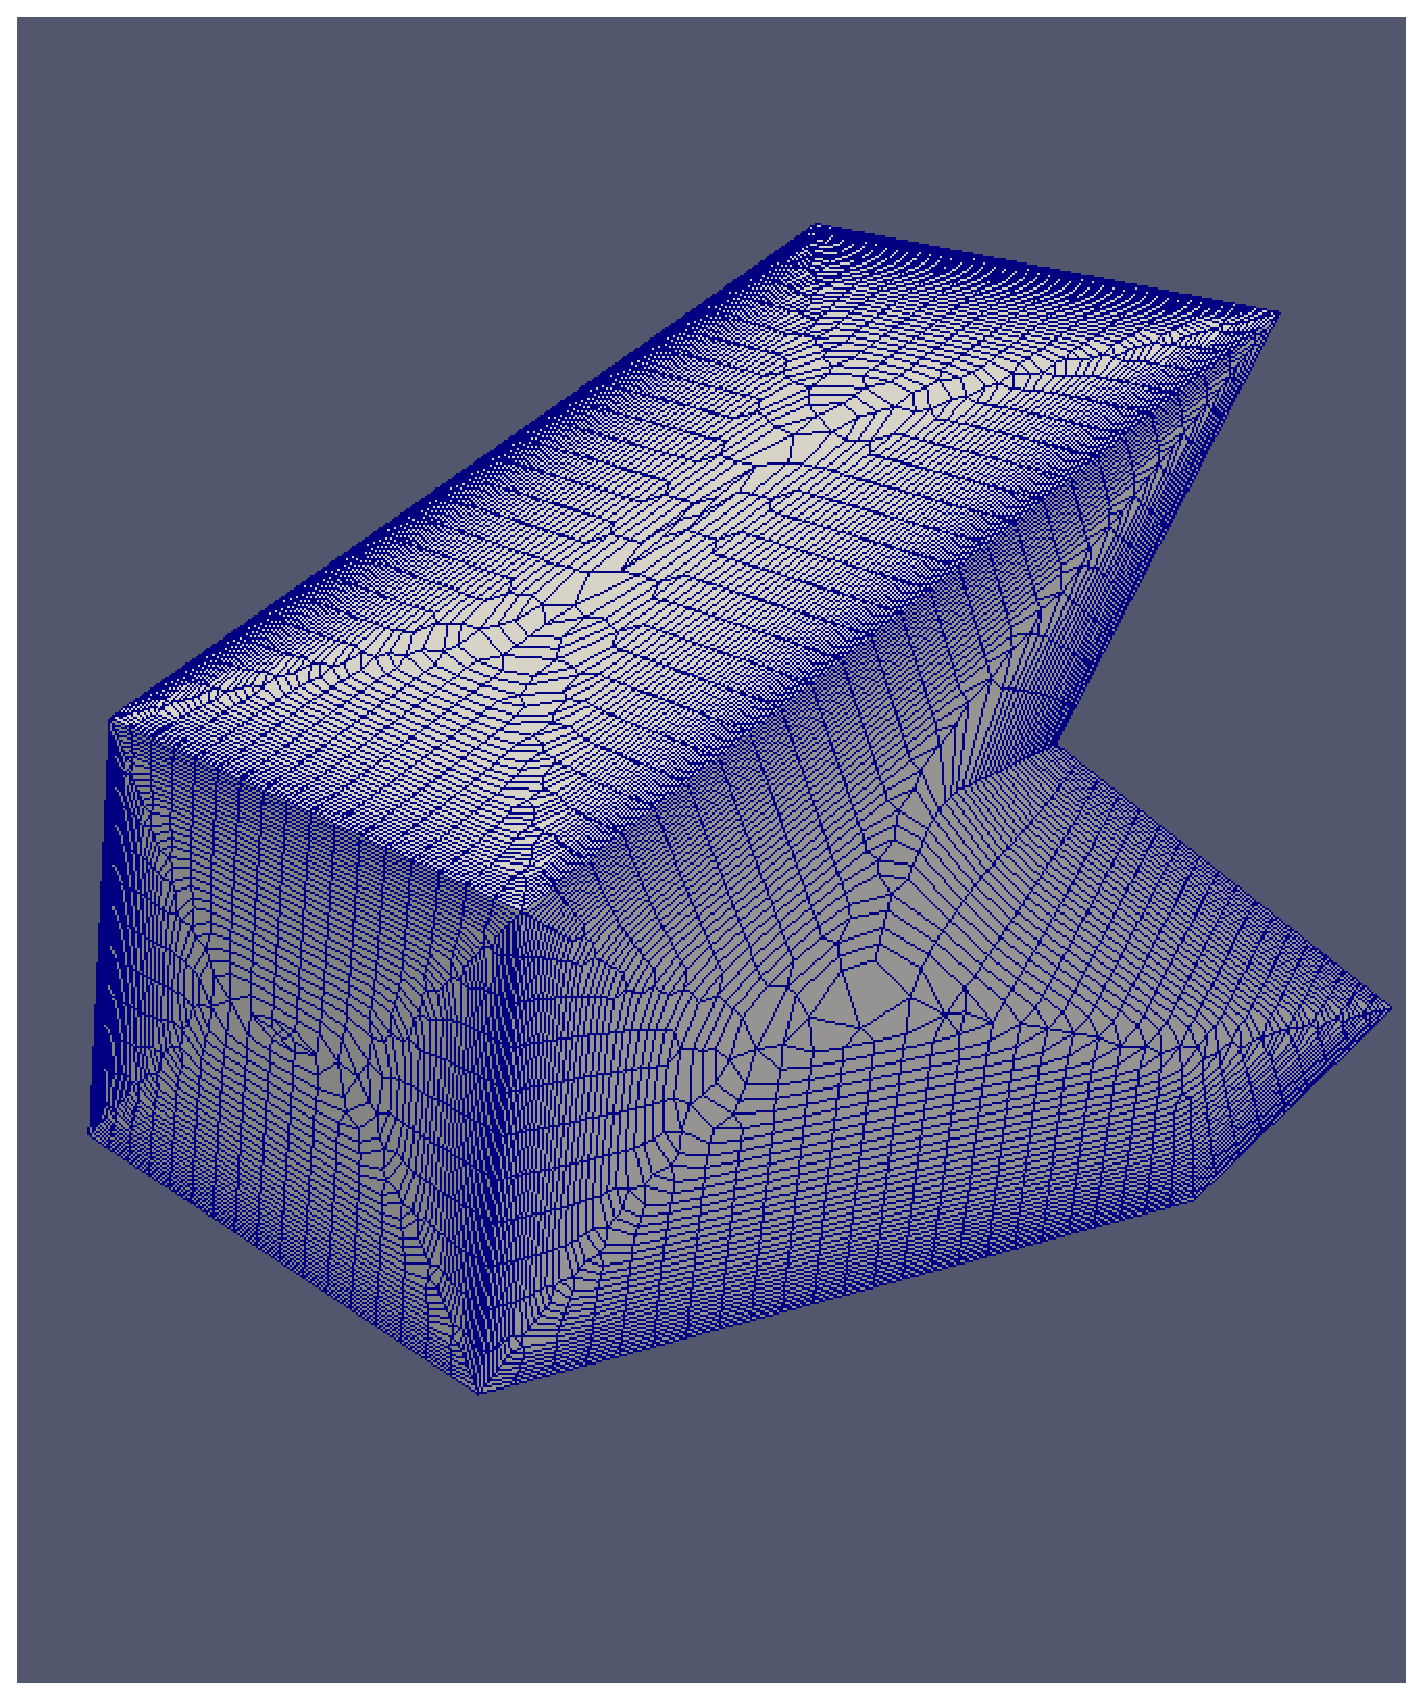
\includegraphics[width = 0.95\linewidth]{img/r/variousAngle-x0.5-g1.04/variousAngle.eps}
		\caption{}
		\label{fig-variousAngle-low}
	\end{subfigure}%
	\begin{subfigure}{0.5\textwidth}
		\centering
		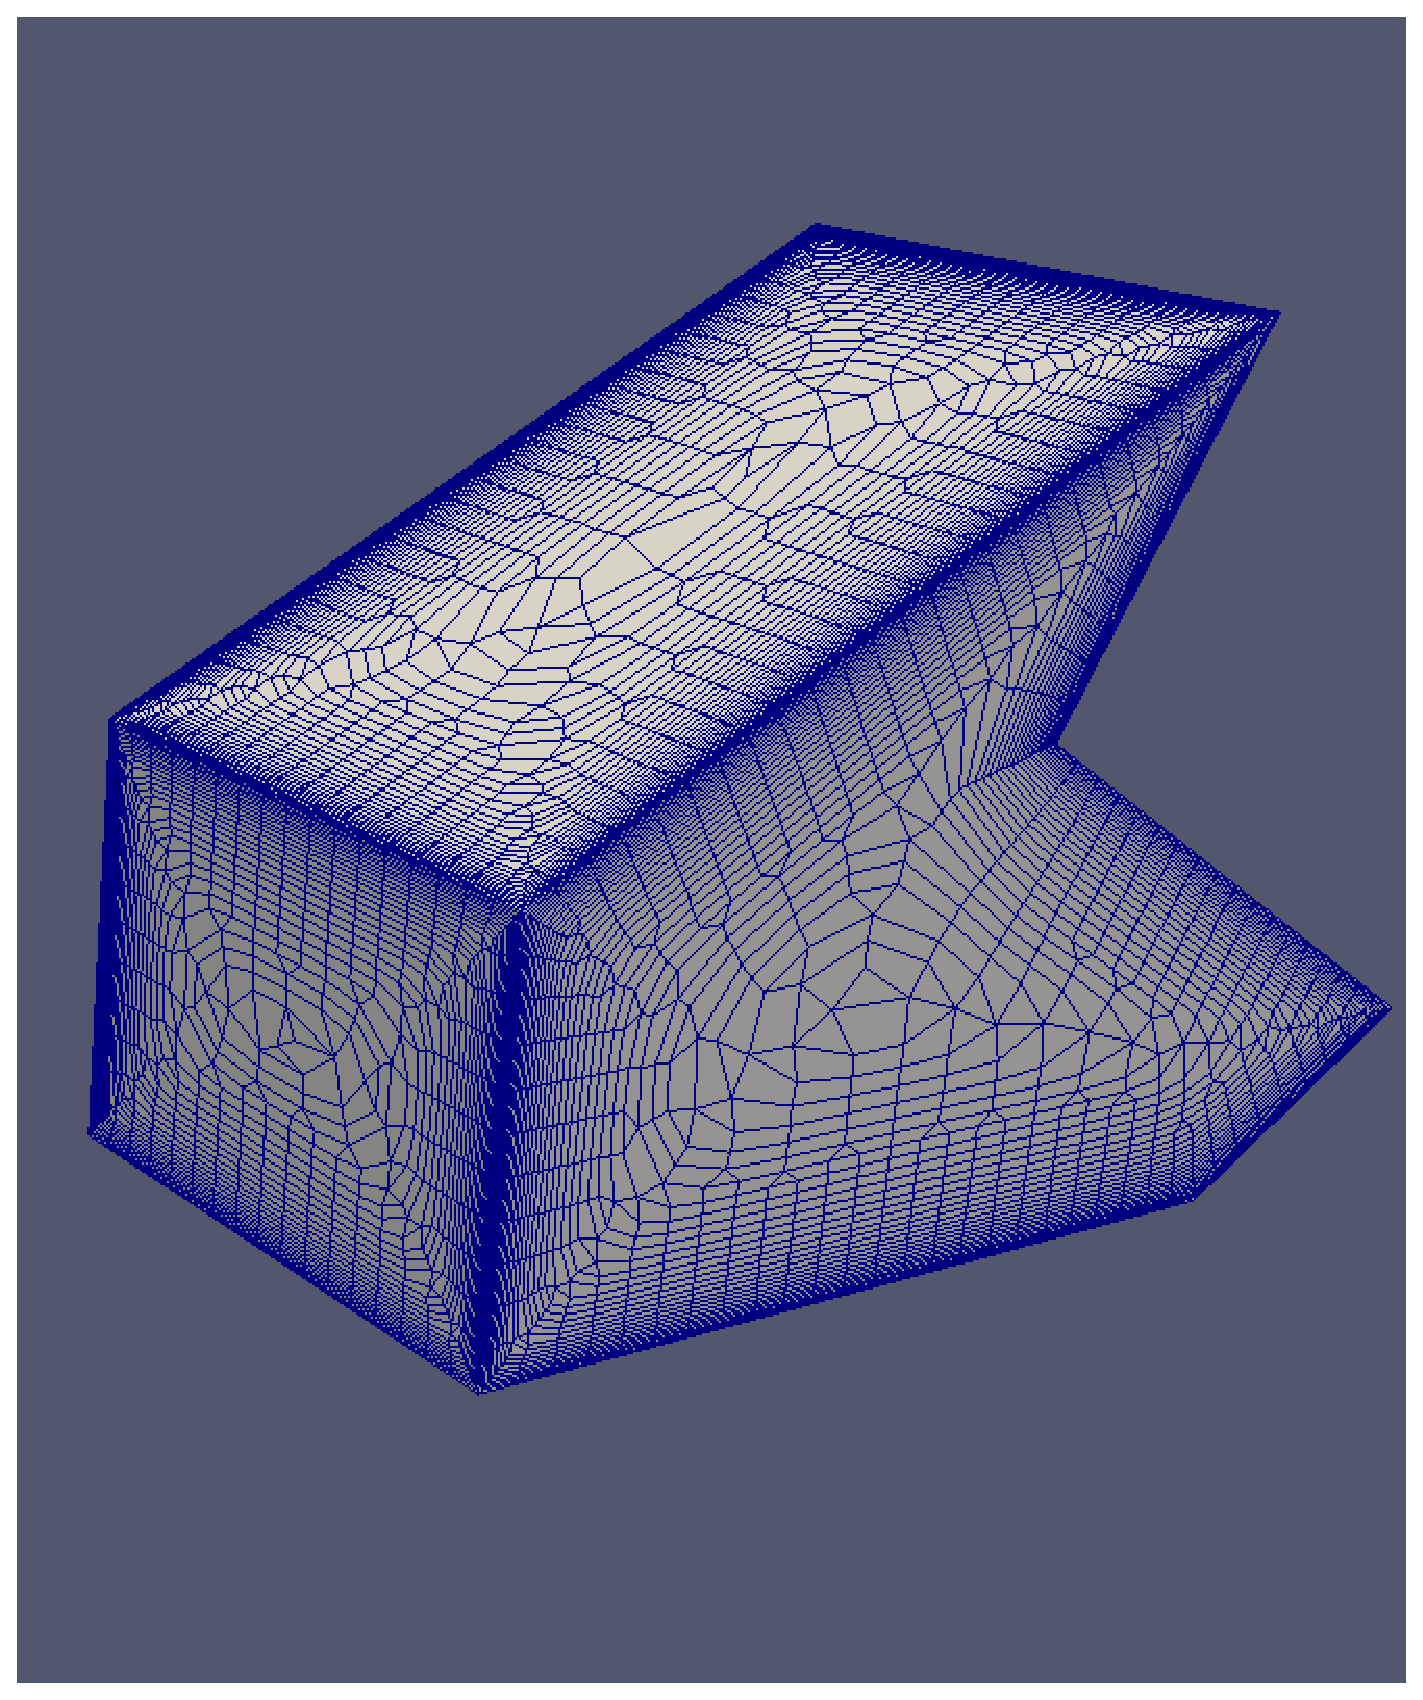
\includegraphics[width=0.95\linewidth]{img/r/variousAngle-x0.3-g1.08/variousAngle.eps}
		\caption{}
		\label{fig-variousAngle-high}
	\end{subfigure}
	\begin{subfigure}{0.5\textwidth}
		\centering
		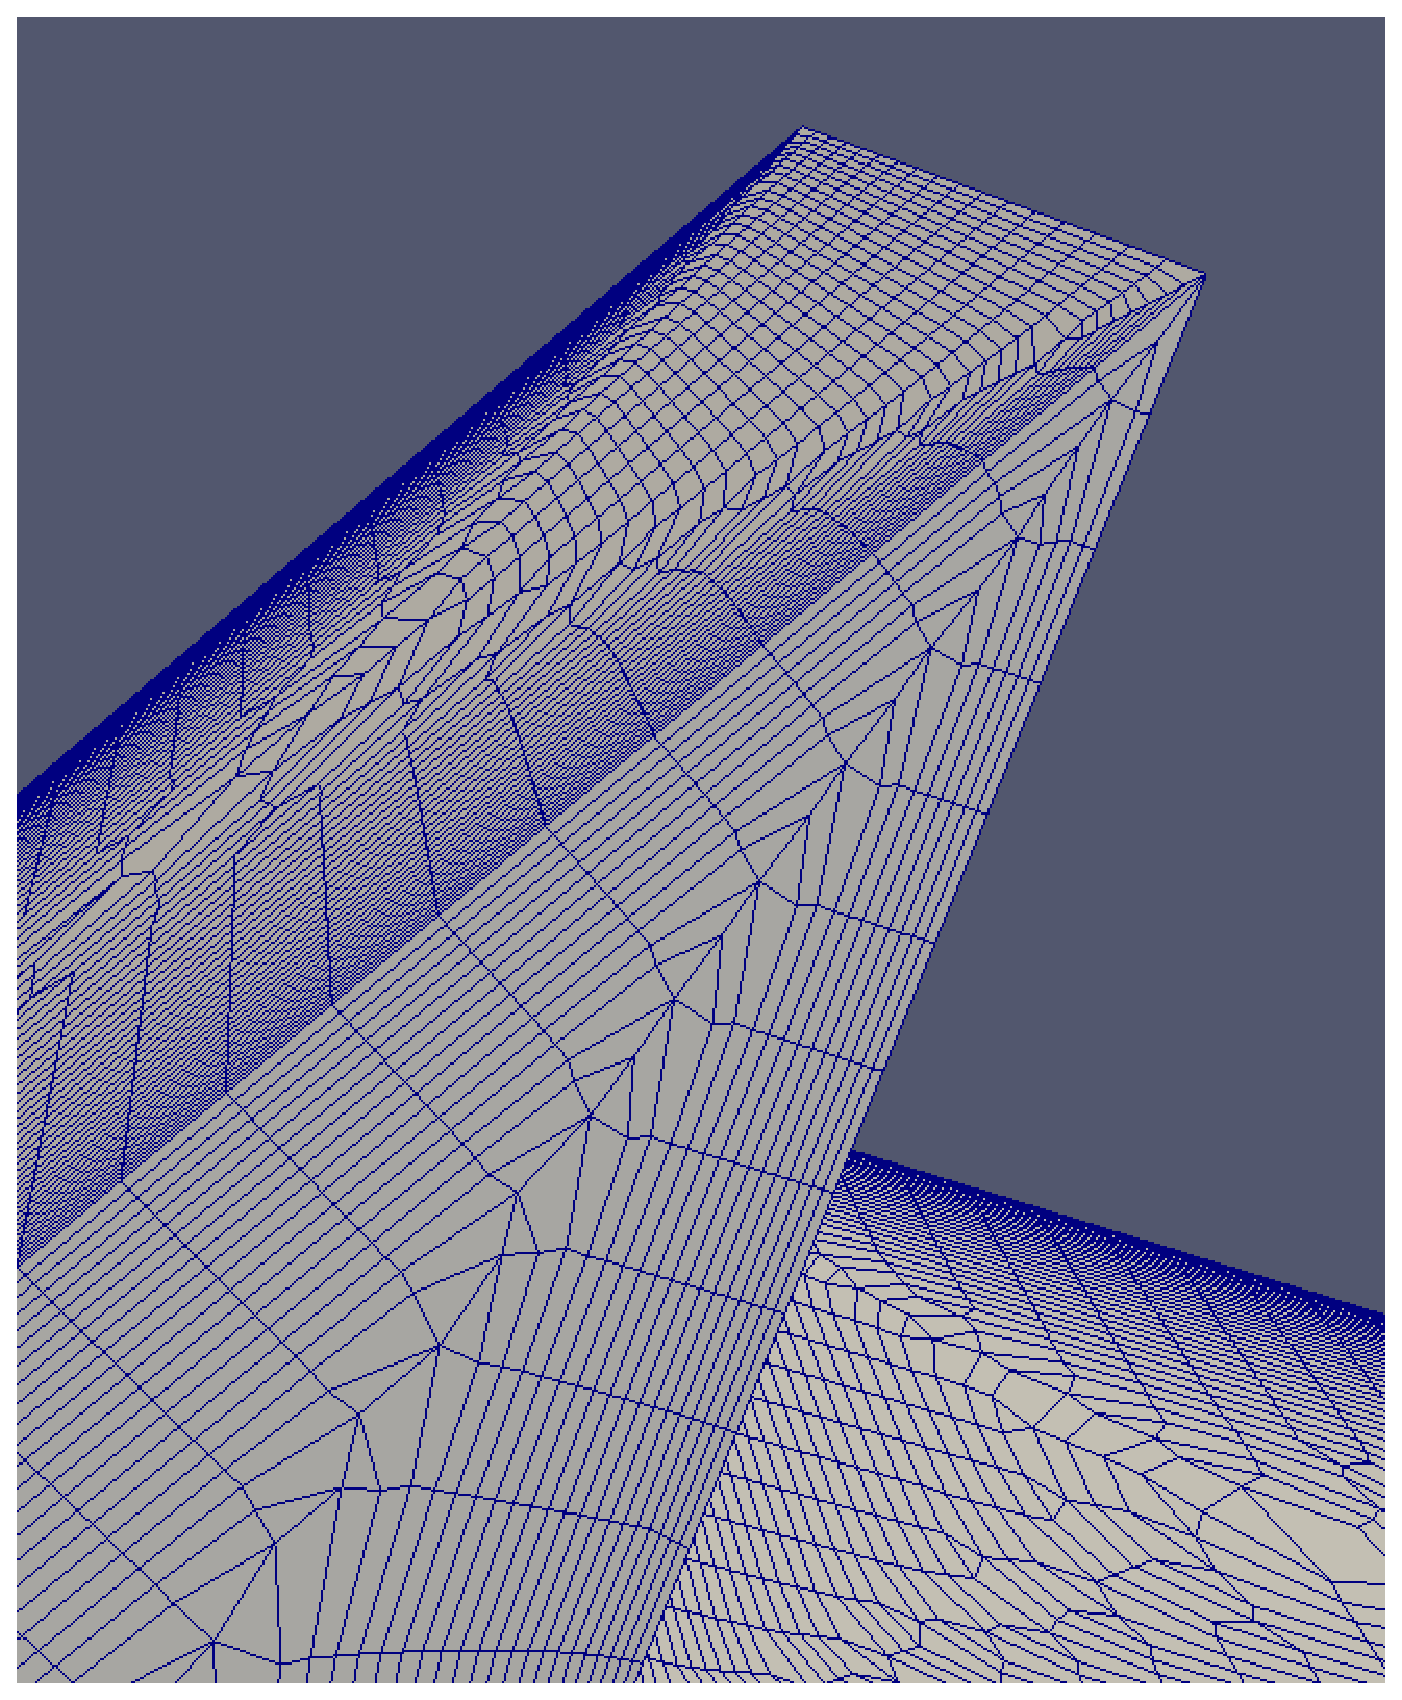
\includegraphics[width=0.95\linewidth]{img/r/variousAngle-x0.5-g1.04/corner.eps}
		\caption{}
		\label{fig-variousAngle-corner-low}
	\end{subfigure}%
	\begin{subfigure}{0.5\textwidth}
		\centering
		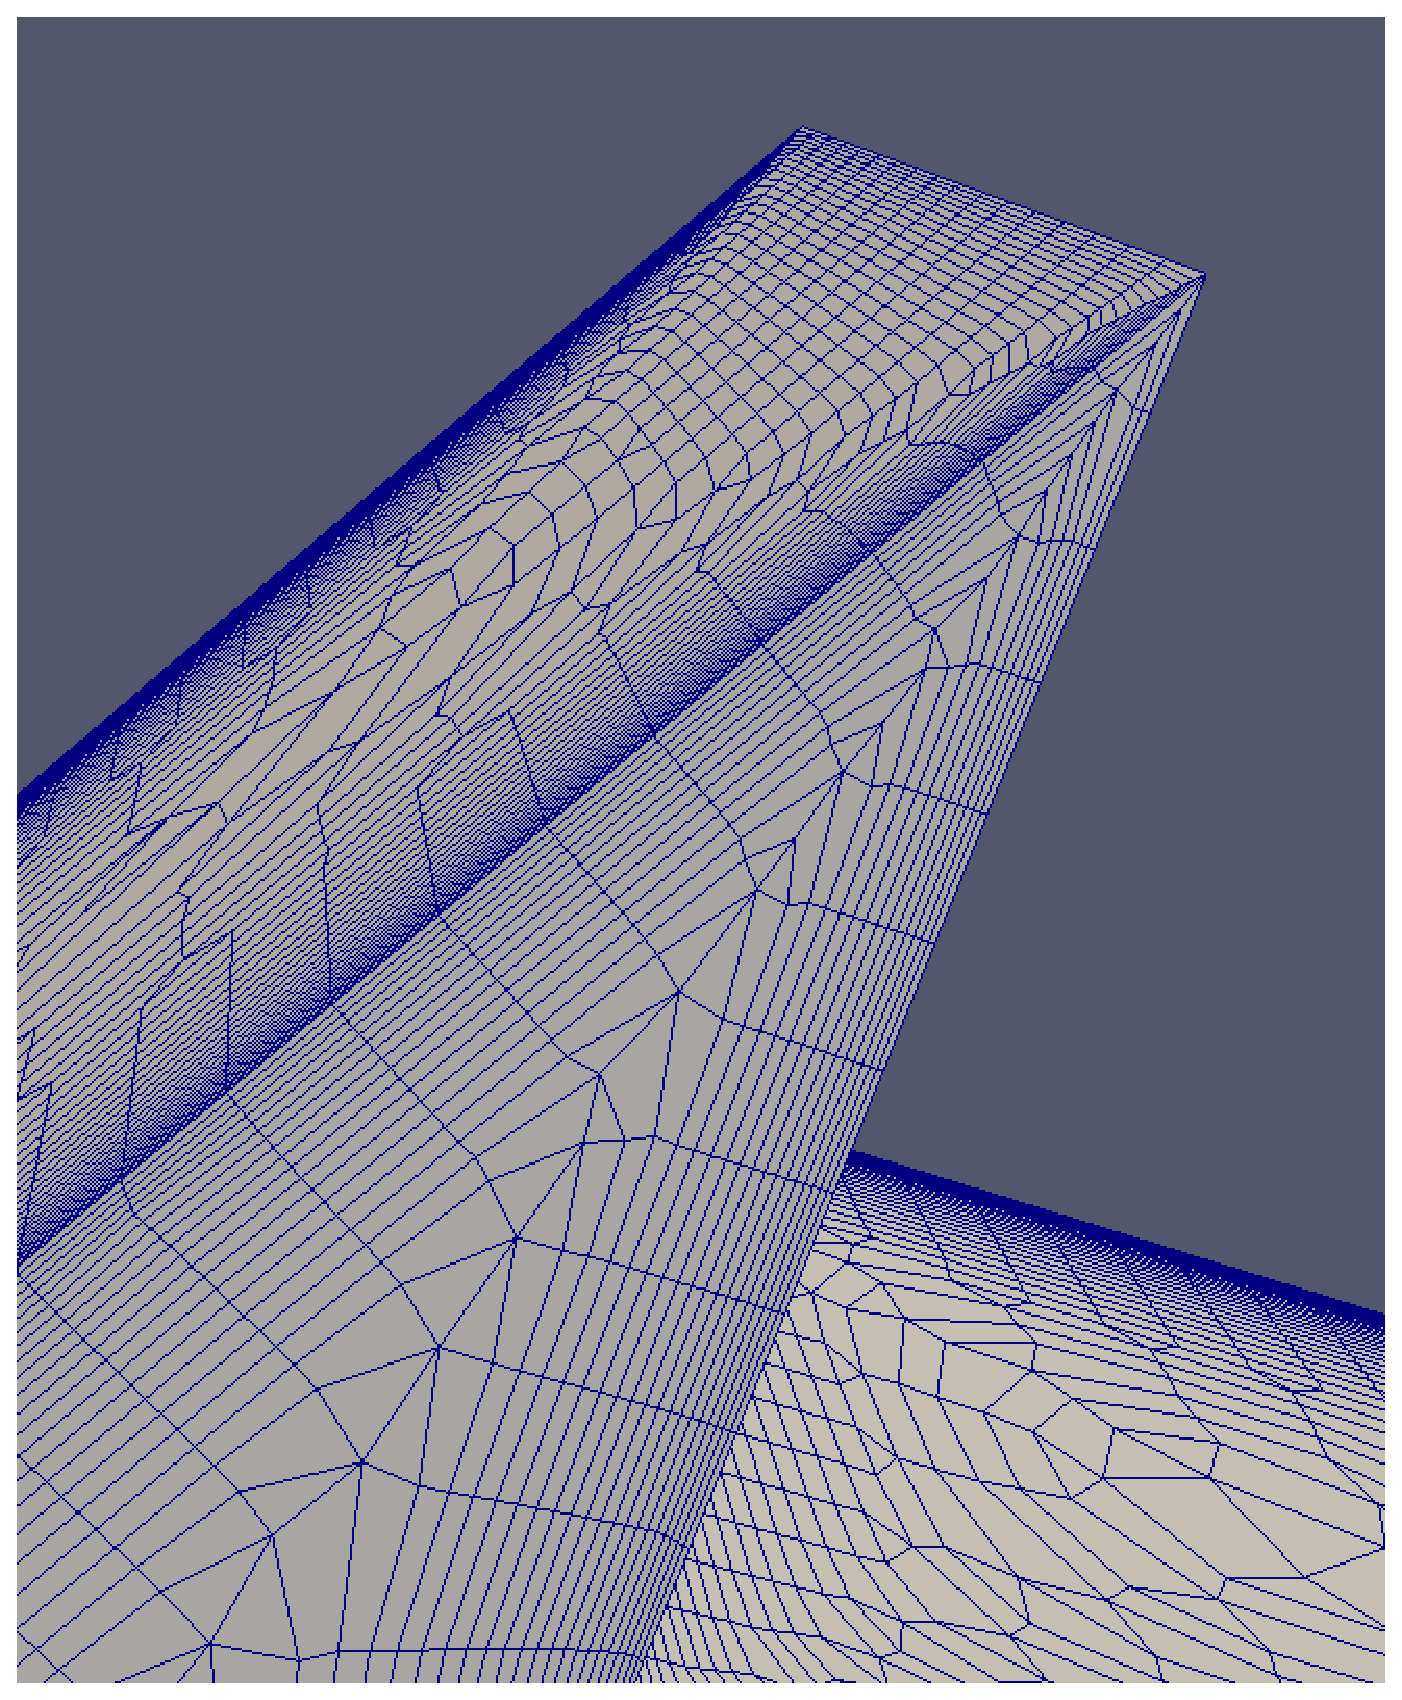
\includegraphics[width=0.95\linewidth]{img/r/variousAngle-x0.3-g1.08/corner.eps}
		\caption{}
		\label{fig-variousAngle-corner-high}
	\end{subfigure}
	\caption[EdamSurf mesh of a geometry with plenty of concave corners (robustness test case 1).]{Geometry with a variety of concave corners at the boundary is meshed with advancing layer surface mesh generation subroutine. On the left, the geometry is meshed with a growth ratio of 1.04 while on the right, it is meshed with a growth ratio of 1.08. The initial extrusion length of the mesh on the right is 40\% less than that on the left. (c) and (d) show the magnified view of a 30$^\circ$ concave corner corresponding to each of the meshes.}
	\label{fig-variousAngle}
\end{figure}

Generating a valid surface mesh for geometries with many concave corners is not a simple task. Vertices situated near a concave corner of the advancing layer encroach on each other, and there is very limited space available to march into. Hence, a robust collision handling subroutine is required to generate a valid mesh at such locations.

To illustrate the robustness of the advancing layer algorithm, especially at the concave corners of the geometry, we run EDAMSurf on a geometry that has surfaces with a variety of concave corners at their boundaries. Figure \ref{fig-variousAngle} shows the resultant meshes generated on such a geometry for two growth ratios: 1.04 and 1.08. The geometry consists of a planar surface with six corners extruded normal to the surface. The concave corners on the geometry range from a 90$^\circ$ corner to a 30$^\circ$ corner.

\begin{figure}
	\centering
	\begin{subfigure}{0.5\textwidth}
		\centering
		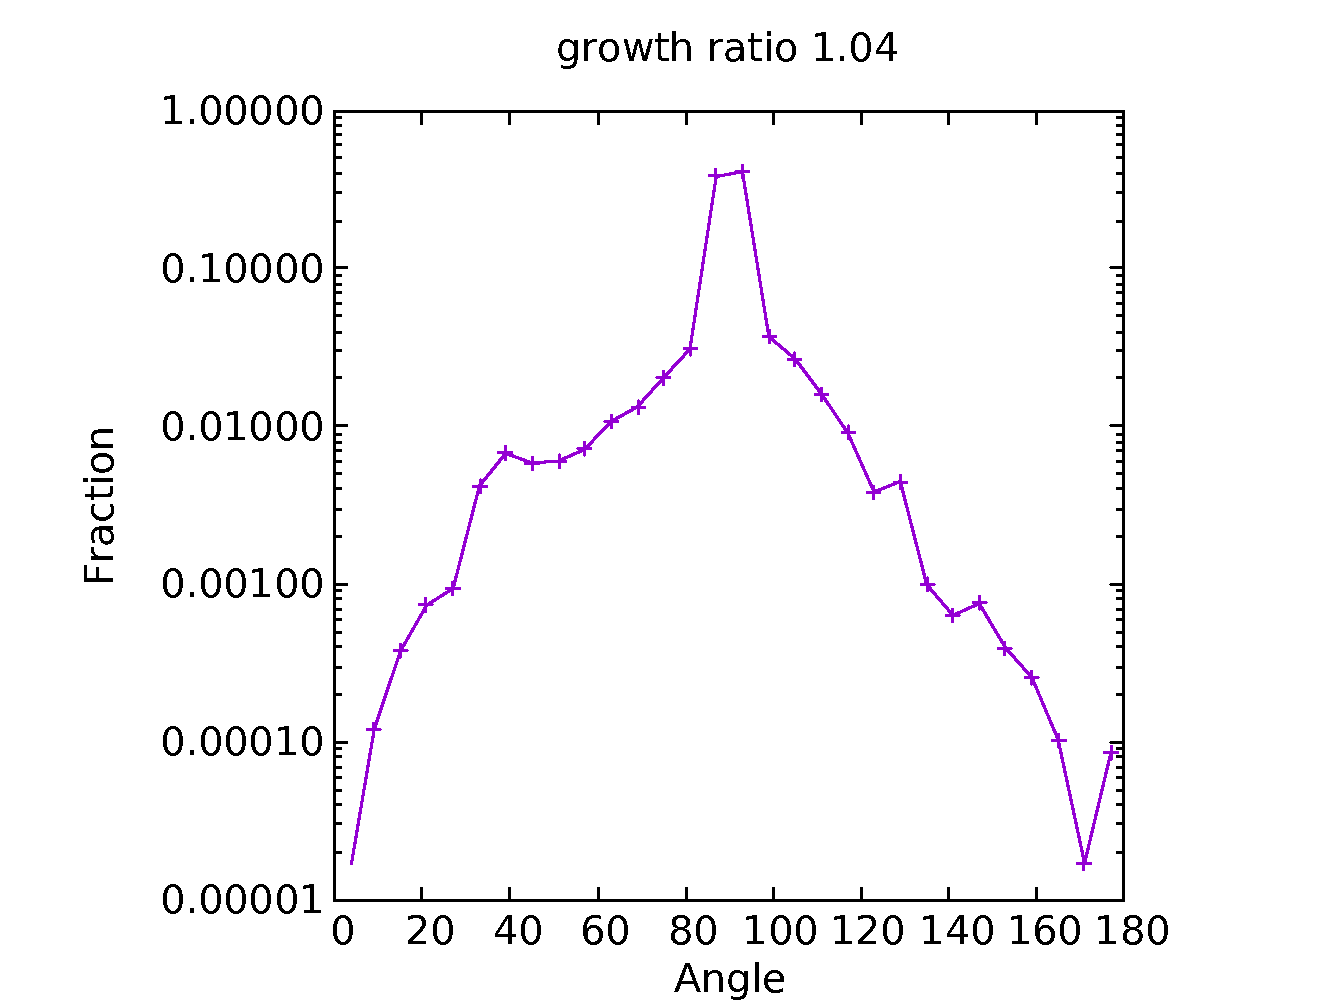
\includegraphics[width=0.9\linewidth]{img/r/variousAngle-x0.5-g1.04/angleDistribution.pdf}
		\caption{}
		\label{fig-va-dist-low}
	\end{subfigure}%
	\begin{subfigure}{0.5\textwidth}
		\centering
		\includegraphics[width = 0.9\linewidth]{img/r/variousAngle-x0.3-g1.08/angleDistribution.pdf}
		\caption{}
		\label{fig-va-dist-high}
	\end{subfigure}
	\caption[Quality of EDAMSurf mesh generated for robustness test case 1.]{Distribution of interior angles of the cells for the meshes generated for the geometry with a variety of concave corners (shown in figure \ref{fig-variousAngle}). Most of the angles are in 45$^\circ$-135$^\circ$ range with a very few skinny traingles.}
	\label{fig-variousAngle}
\end{figure}

Surface meshes generated from the geometry can be seen to have the required anisotropic elements at the boundary of the surface. Figure \ref{fig-variousAngle-corner-low} and \ref{fig-variousAngle-corner-high} show magnified view of a 30$^\circ$ concave corner in the mesh. Even though the mesh is advancing from the sharp corner towards the surface interior, it successfully recovers the front at each iteration of the advancing layer routine. Also, the quality of the mesh elements remains consistent as the mesh grows from the boundary. Additionally, the boundary topology is successfully retained several layers into the advancing layer mesh generation process. Hence, EDAMSurf is successful in marching out concave corners for the given geometry.

Figure \ref{fig-variousAngle} shows the distribution of interior angles of the mesh elements of these meshes. In this example, the majority of the angles in the mesh are around 90$^\circ$. The distribution is a bit flattened out. This is due to the concave corners in this geometry. Still, the number of skinny triangles in the mesh is negligible. The percentage of quads generated for the low growth ratio mesh is 96.43\% and for the high growth ratio mesh is 95.82\%. Hence, even though the mesh has many concave corners, more than 95\% of the mesh elements are non-simplicial quad elements.

\section{Robustness Test 2 --- Diverse Topology Handling}

In the previous section, we saw how EDAMSurf is capable of meshing geometries with sharp corners. We test our advancing layer mesh generation subroutine for one more case. Here, we input a geometry that is shaped like a mechanical joint. The solid body has 10 surfaces. Each of the surfaces is different from the rest. There are curved as well as flat surfaces. The surfaces of the mechanical part test EDAMSurf with a variety of surface patches or segmented sub surfaces.

Figure \ref{fig-joint} shows the output mesh generated from the mechanical joint from several angles. Highly stretched elements are created at the boundary of the geometry. As the mesh grows towards the surface interior, the advancing layer grows in size, hence generating the required level of anisotropy at the boundaries. The aspect ratio for this mesh at the boundary varies with the boundary vertices but is set to be around 9-10. This illustrates that the mesh generator is capable of handling a variety of surface topologies. The mesh contains 45,740 cells and 45,020 points. There are 44,304 quadrilateral elements in the mesh while the number of triangular elements is just 1436.

\begin{figure}[hbt!]
	\centering
	\begin{subfigure}{.33\textwidth}
		\centering
		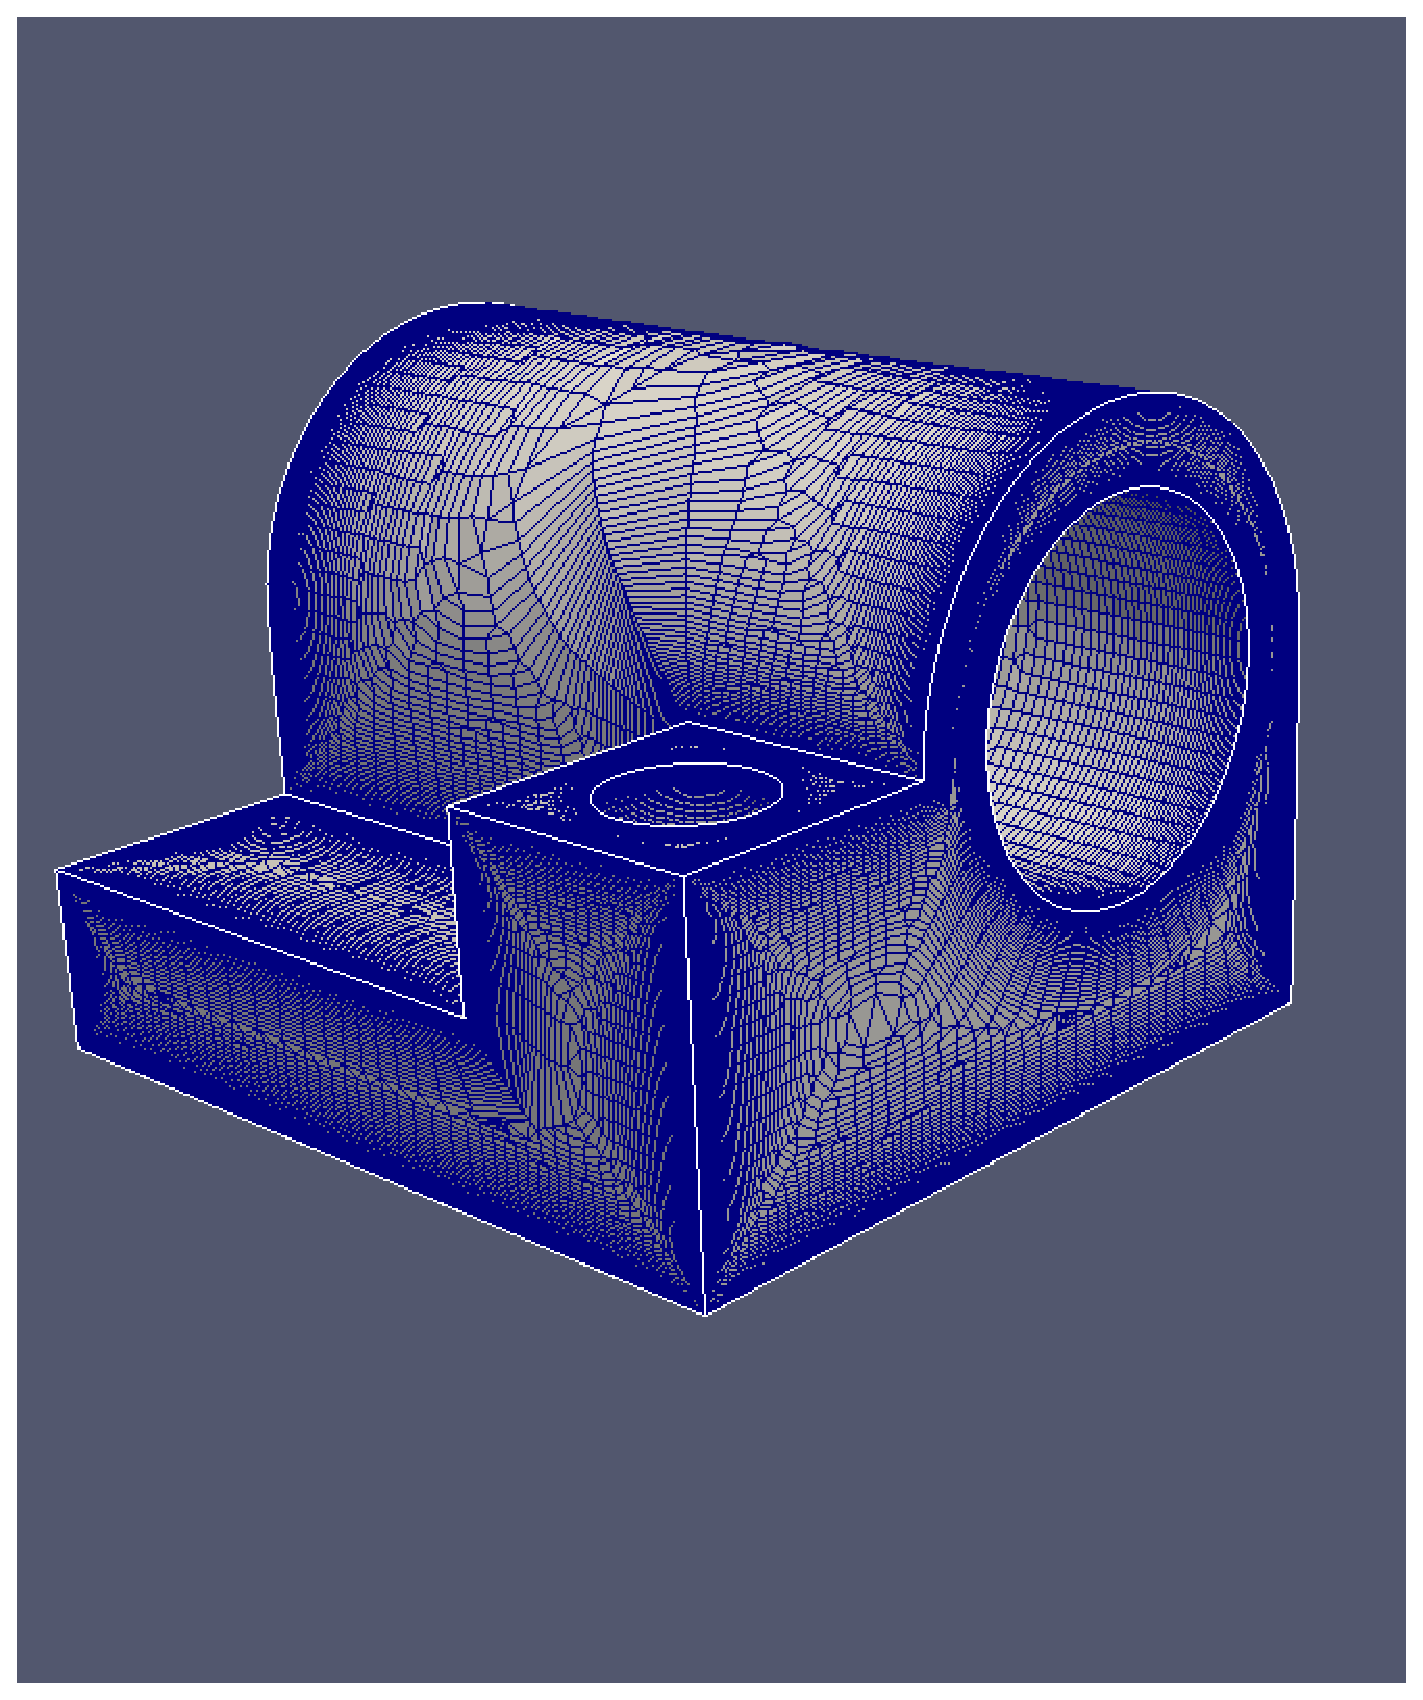
\includegraphics[width=.9\linewidth]{img/r/joint-x0.004-g1.04-a5/oblique.eps}
		\caption{}
		\label{fig-joint-oblique}
	\end{subfigure}%
	\begin{subfigure}{.33\textwidth}
		\centering
		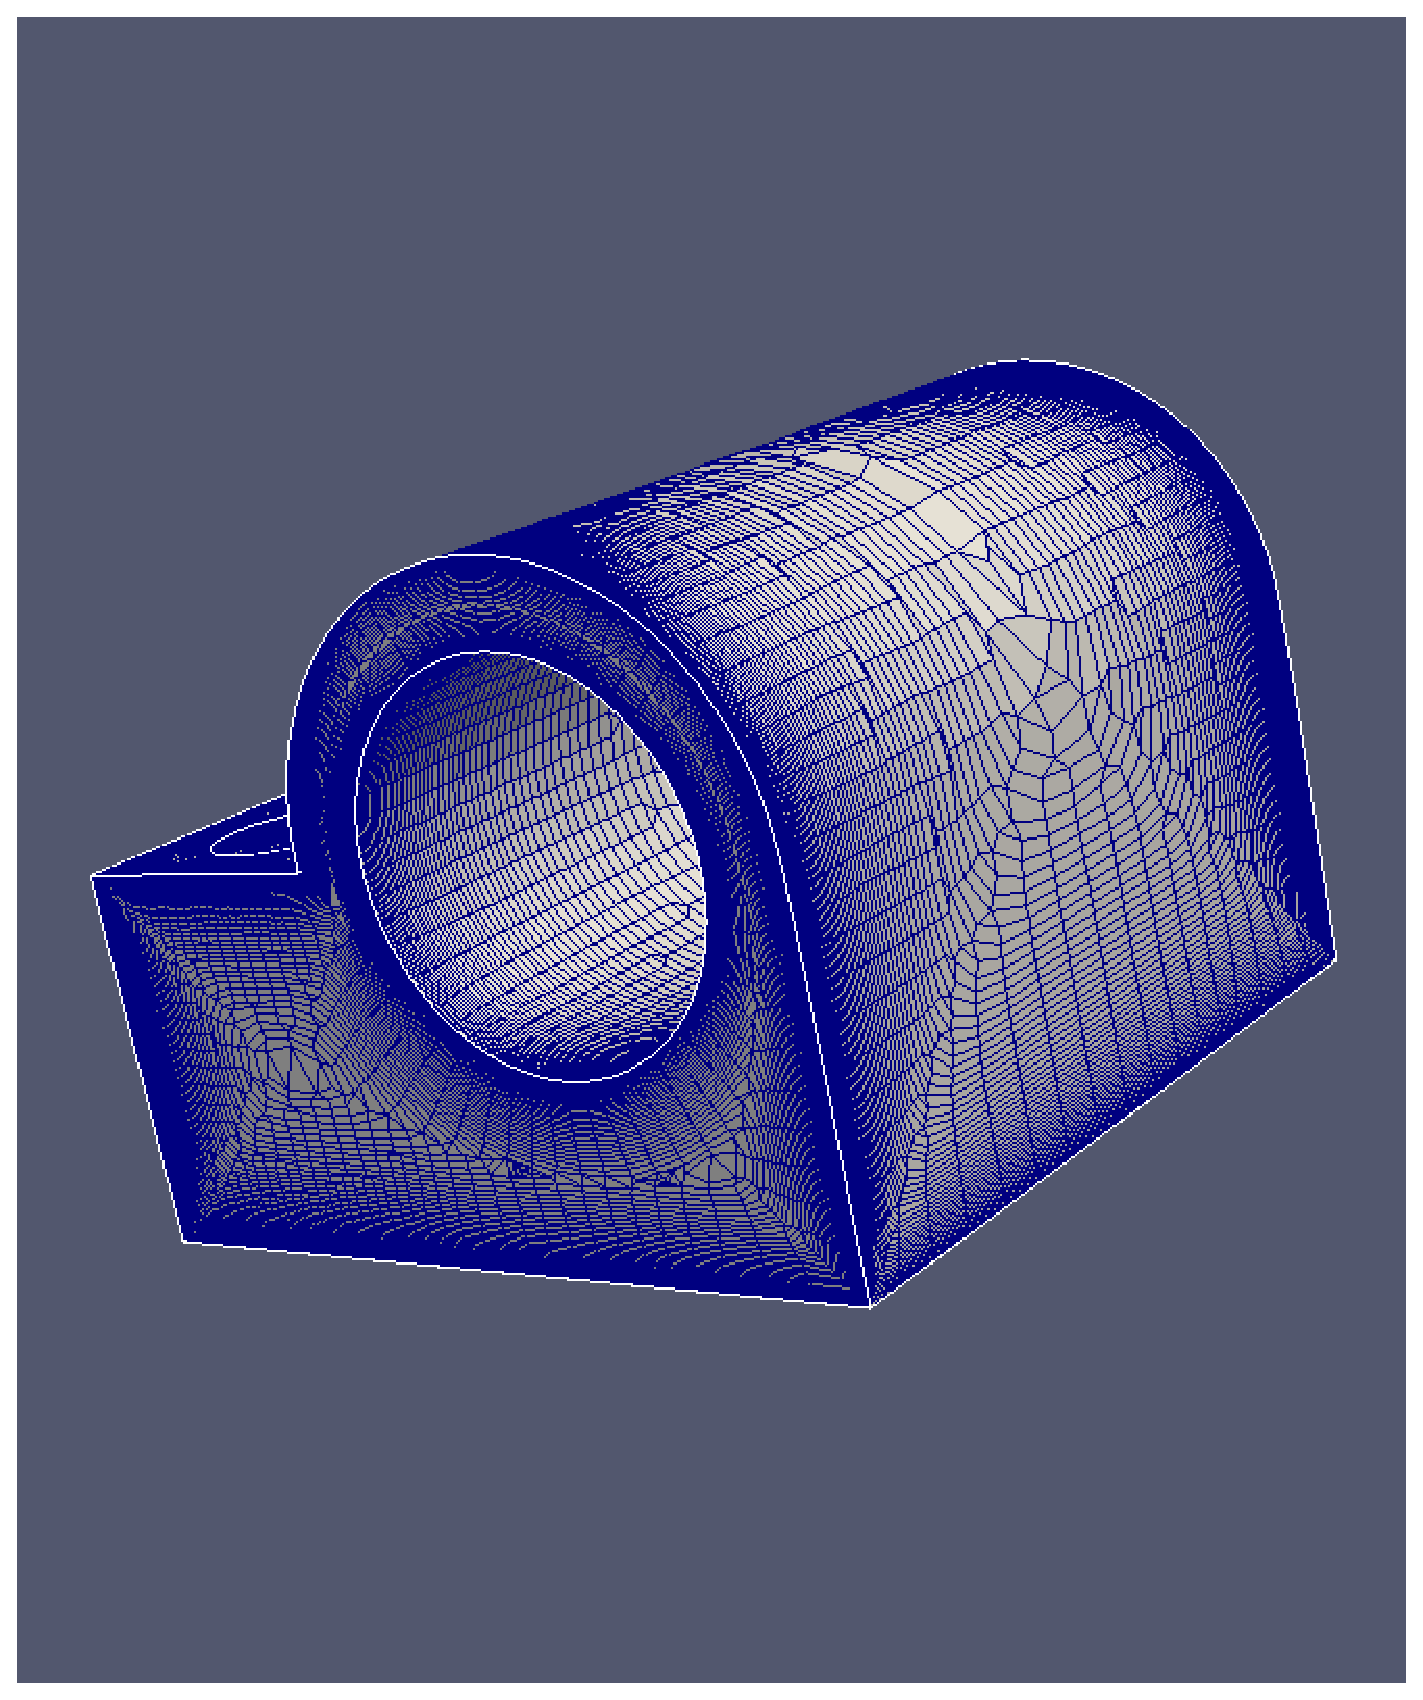
\includegraphics[width=.9\linewidth]{img/r/joint-x0.004-g1.04-a5/oblique1.eps}
		\caption{}
		\label{fig-joint-oblique1}
	\end{subfigure}%
	\begin{subfigure}{.33\textwidth}
		\centering
		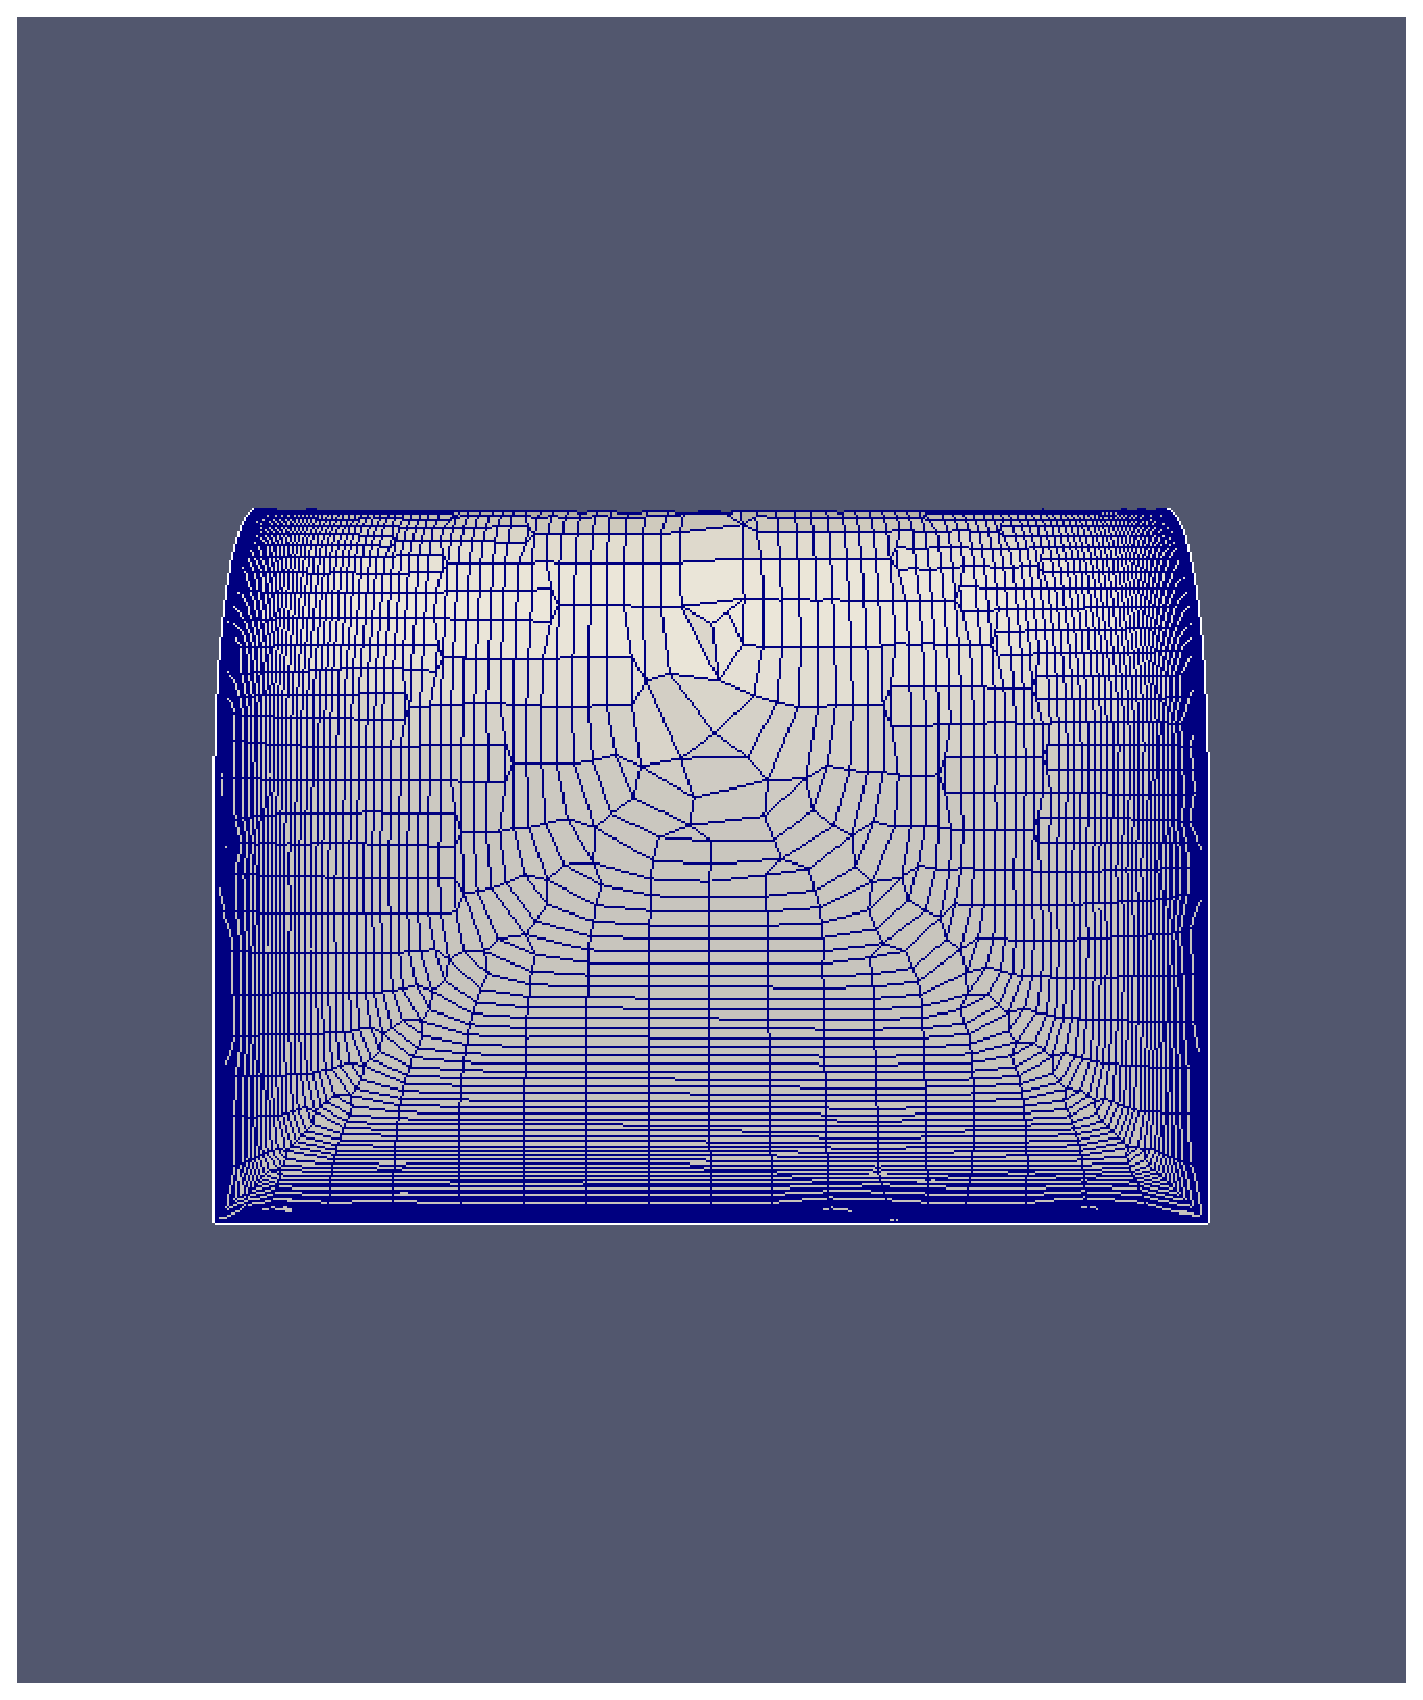
\includegraphics[width=.9\linewidth]{img/r/joint-x0.004-g1.04-a5/side.eps}
		\caption{}
		\label{fig-joint-side}
	\end{subfigure}
	\begin{subfigure}{.33\textwidth}
		\centering
		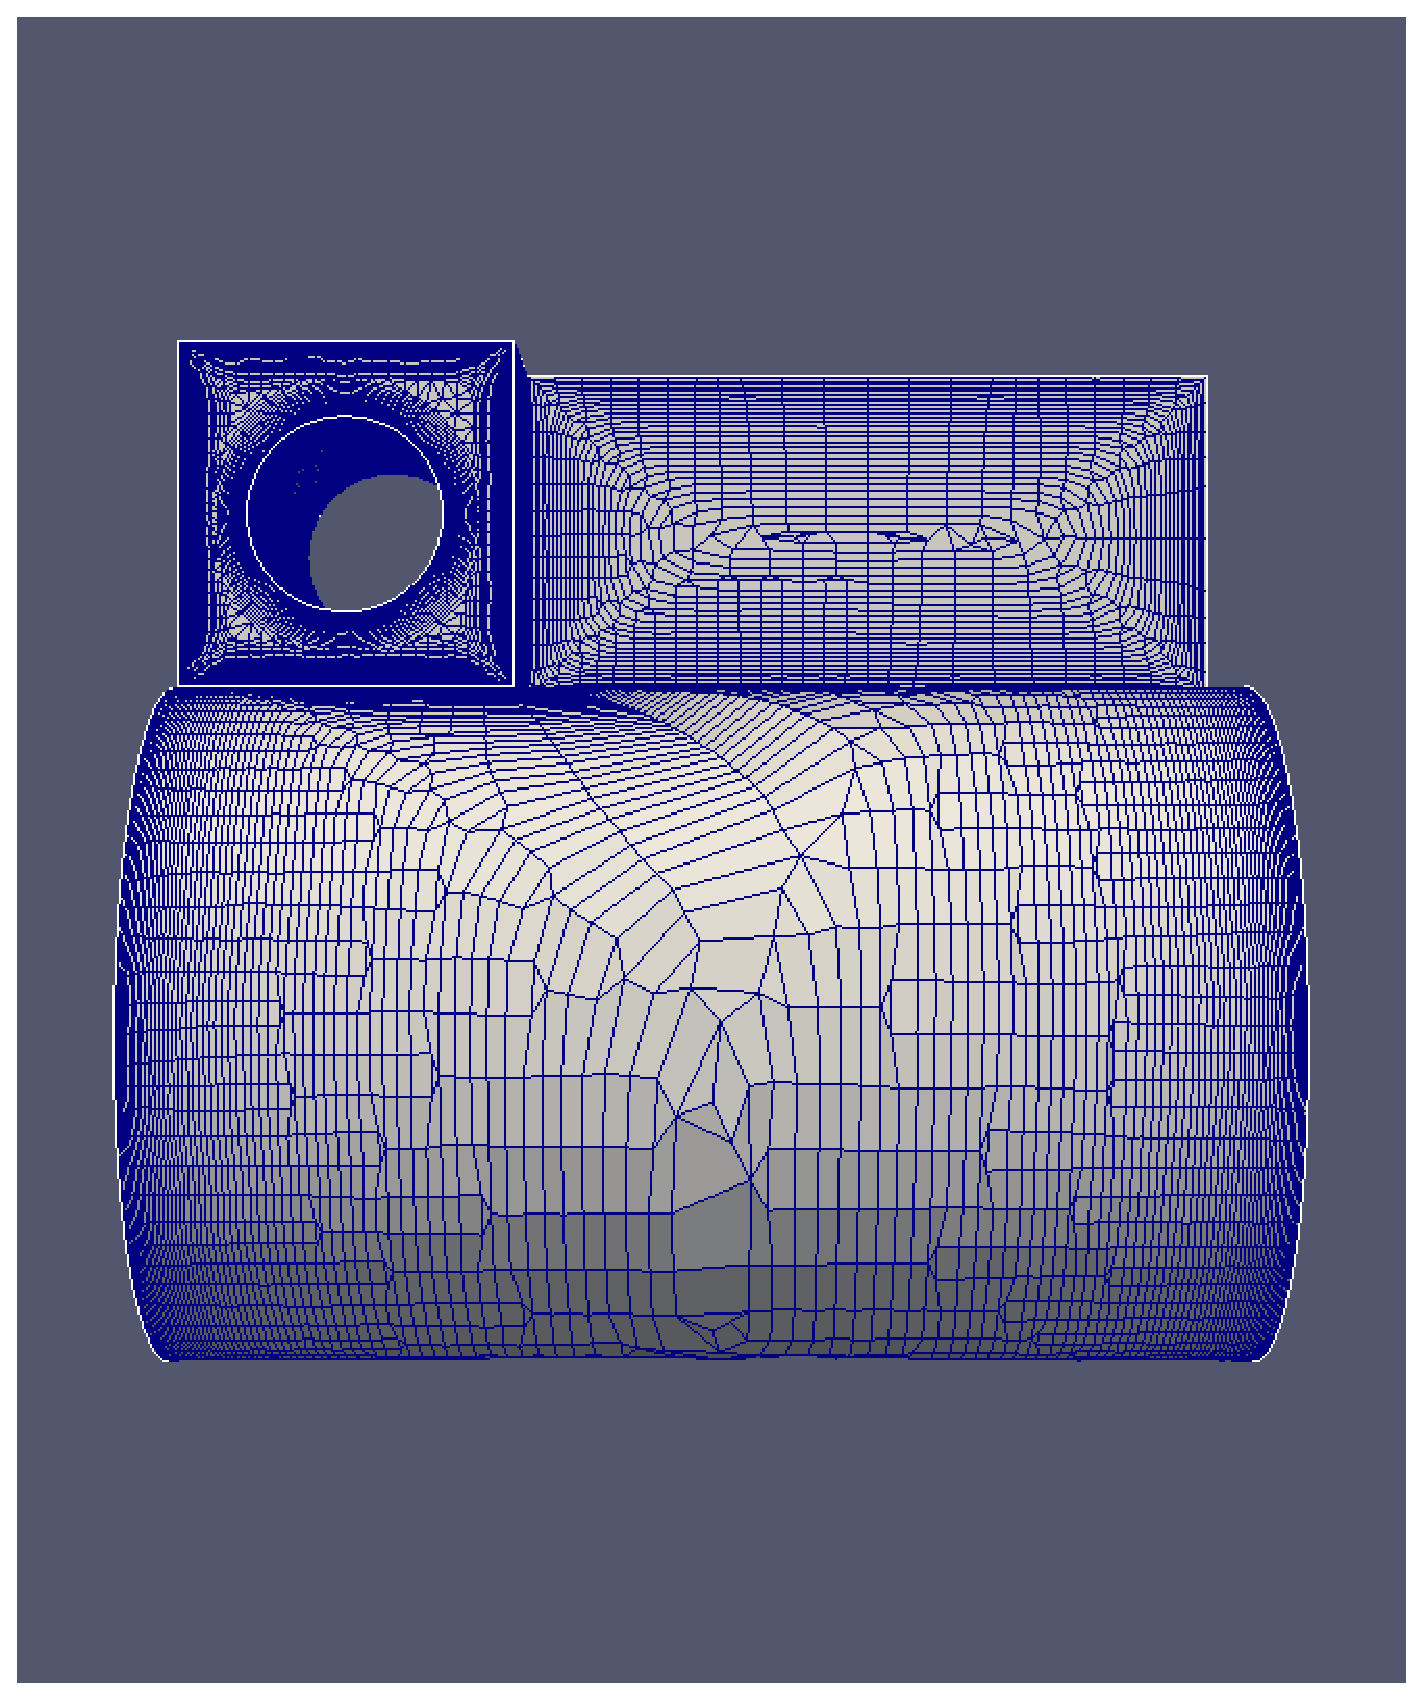
\includegraphics[width=.9\linewidth]{img/r/joint-x0.004-g1.04-a5/top.eps}
		\caption{}
		\label{fig-joint-top}
	\end{subfigure}%
	\begin{subfigure}{0.33\textwidth}
		\centering
		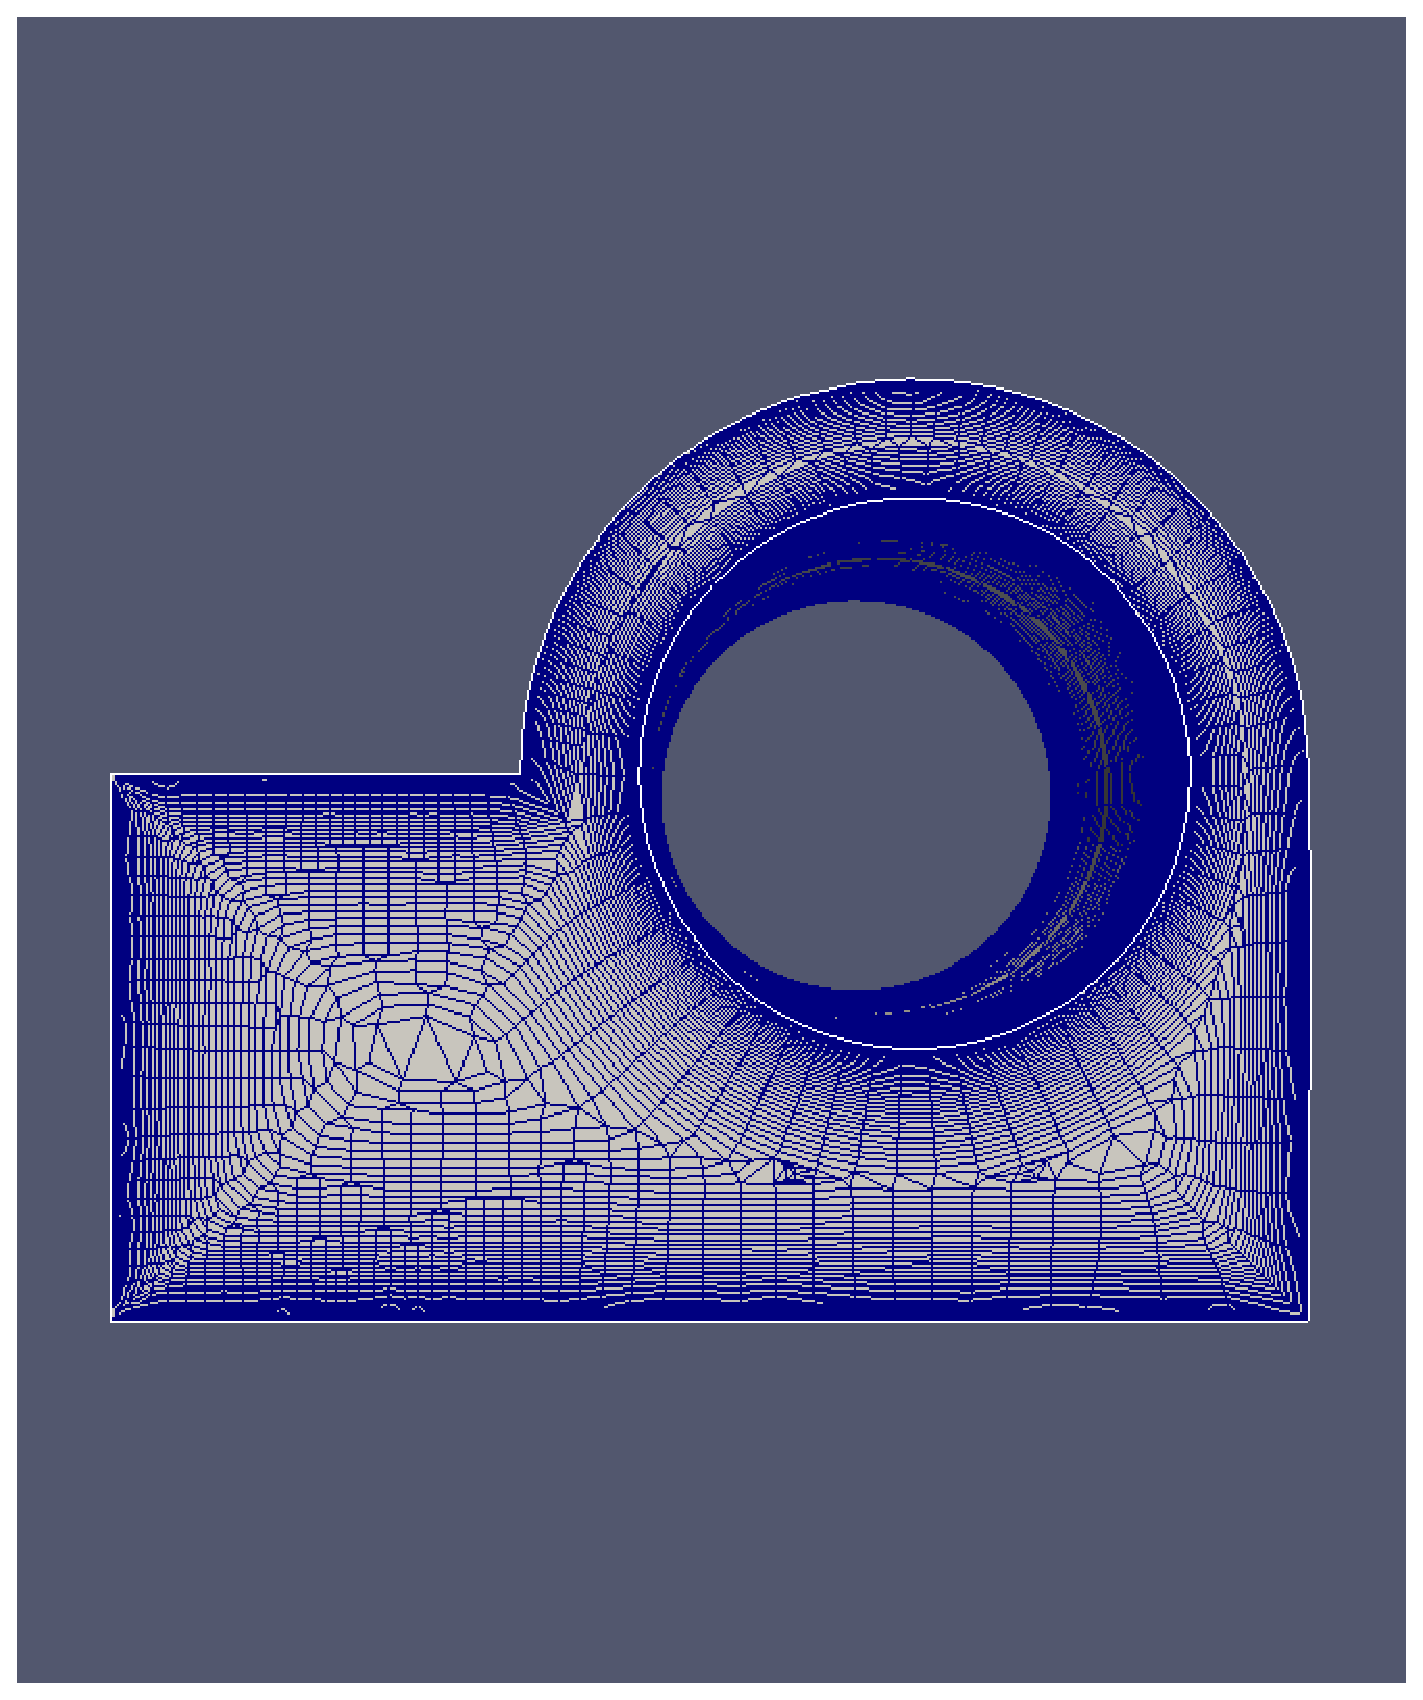
\includegraphics[width=0.9\linewidth]{img/r/joint-x0.004-g1.04-a5/front.eps}
		\caption{}
		\label{fig-joint-front}
	\end{subfigure}%
	\begin{subfigure}{0.33\textwidth}
		\centering
		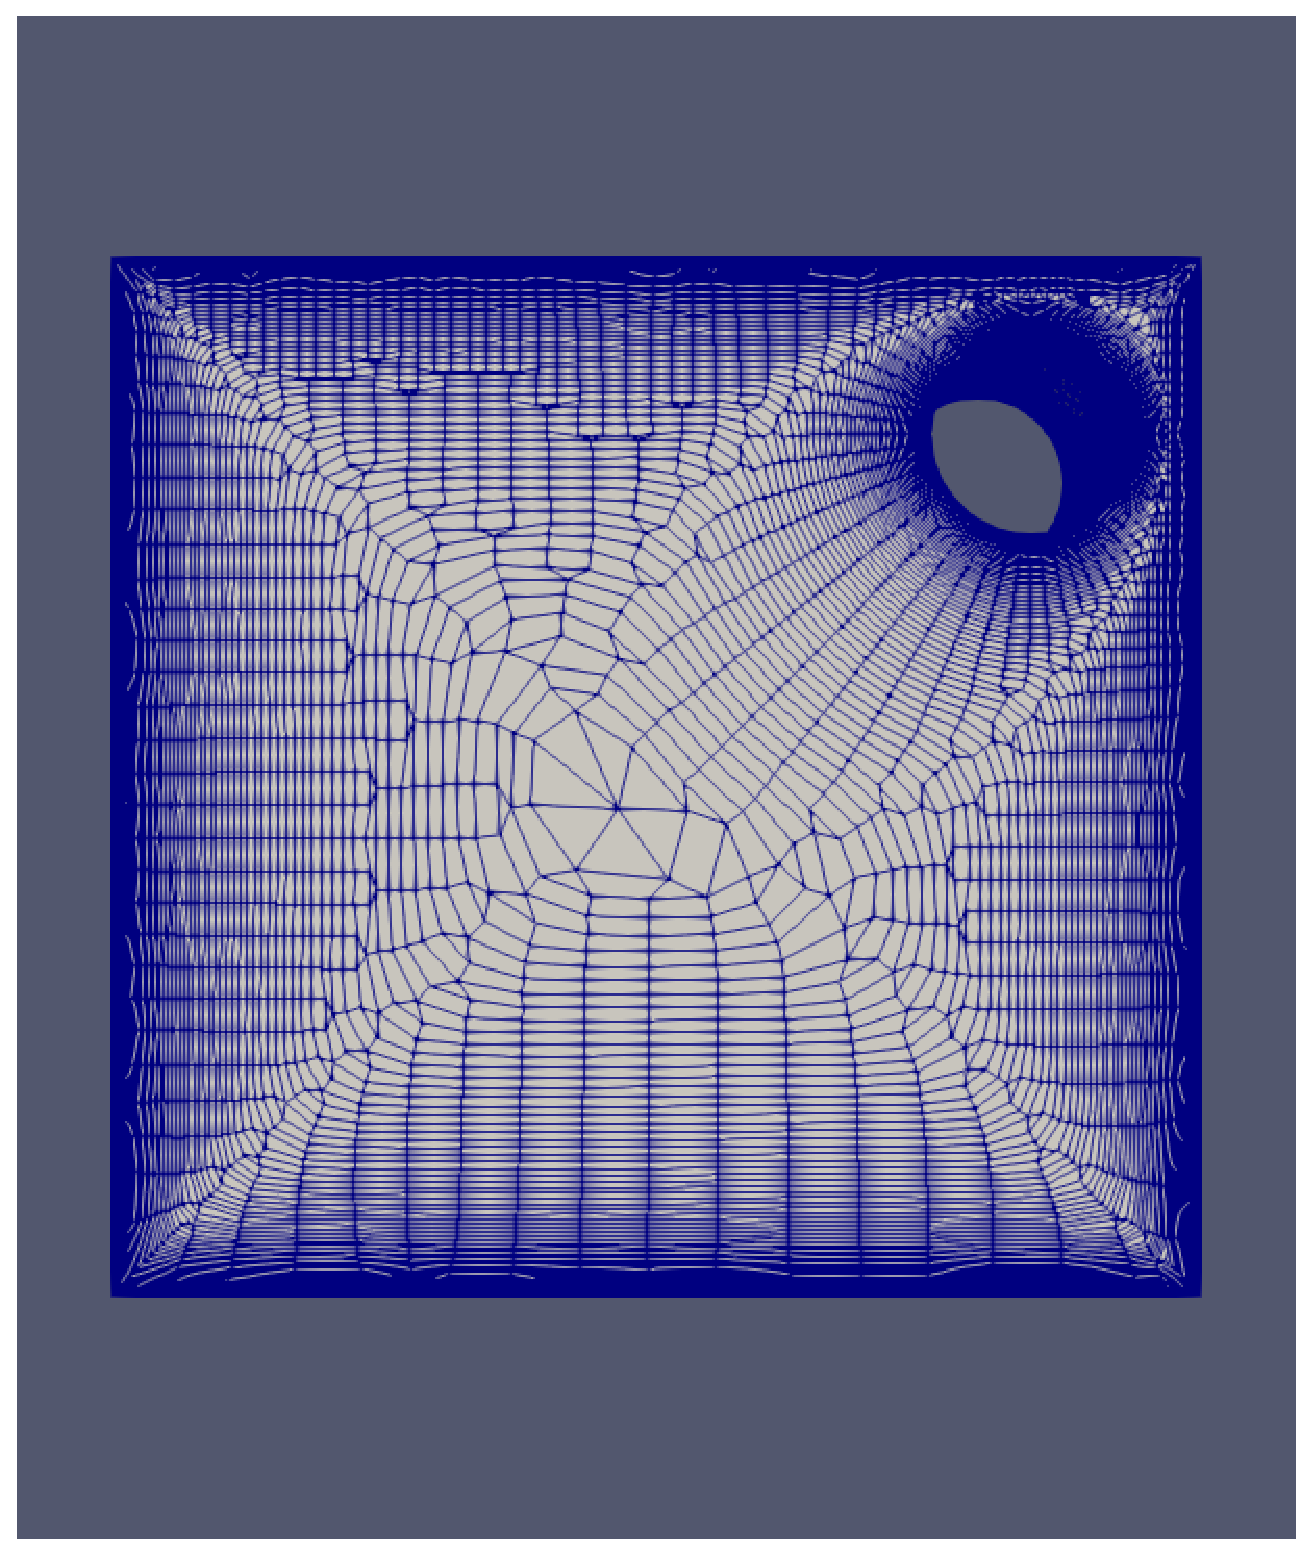
\includegraphics[width=0.9\linewidth]{img/r/joint-x0.004-g1.04-a5/bottom.eps}
		\caption{}
		\label{fig-joint-bottom}
	\end{subfigure}
	\caption[EDAMSurf mesh of a mechanical part (robustness test case 2).]{Geometry shown in Figure \ref{fig-surfSegment} is meshed using the advancing layer surface mesh generation routine. The algorithm is able to tackle a variety of surface topologies while generating anisotropic meshes. Given level of anisotropy can be obtained on the boundaries of the mesh with the algorithm.}
	\label{fig-joint}
\end{figure}

In Figure \ref{fig-closeUp}, we show close-ups at two locations on the mesh where advancing layers from several boundaries collide in a comparatively limited region. Figure \ref{closeUp1} shows the close-up view of the top of the mechanical part, near the region where the flat section with a cylindrical cutout meets the curved surface at the top. Advancing layers from the circular boundary of the cylindrical cutout and the two straight boundaries of the surface path collide after advancing several layers onto the surface. At each advancing layer, the collision handling subroutine checks for possible encroaching vertices. It stops selected points from marching forward to avoid front collapse and hence finishes the mesh generation process in some regions of the surface patch while continuing the process in the remaining regions.

Another example of a collision between multiple independently advancing marching layers on the surface mesh is shown in figure \ref{closeUp2}. Here, we show the bottom of the mechanical part near the cylindrical cutout. Layers start to march from the circular cutout as well as the rectangular boundary of the bottom surface. There is high anisotropy at these boundary curves. As the layers march onto the surface, we see that the aspect ratio of the mesh elements gradually drops. One by one, the points on an advancing front which encroach on other points are stopped from marching. This is done until the point when there are no more vertices left on the advancing front to march further. This completes the mesh generation process. These figures demonstrate the robustness of EDAMSurf. Hence, it is possible to mesh a surface with varied topological features using our mesh generation scheme.

\begin{figure}
	\centering
	\begin{subfigure}{.5\textwidth}
		\centering
		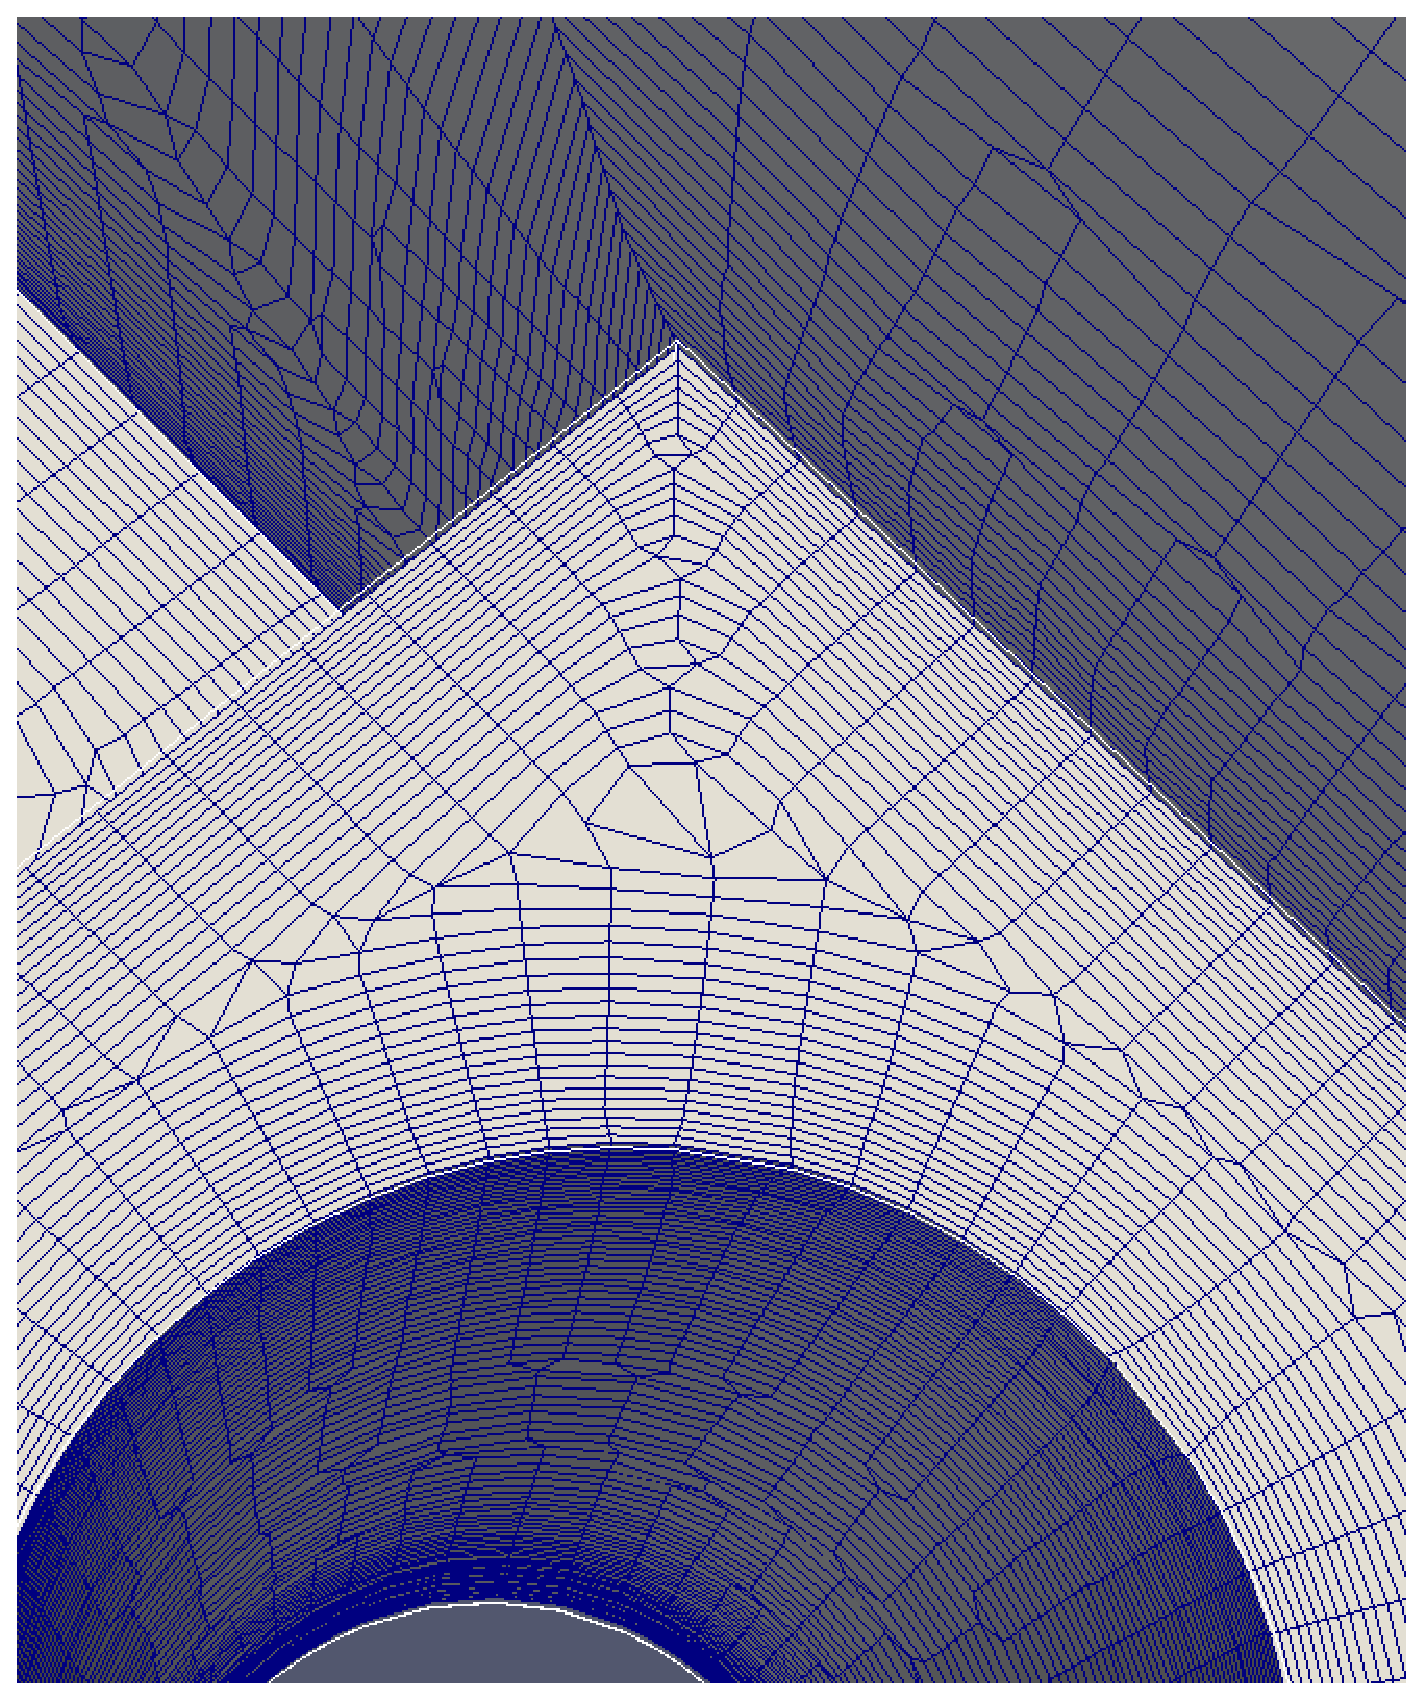
\includegraphics[width=0.9\linewidth]{img/r/joint-x0.004-g1.04-a5/closeUp.eps}
		\caption{}
		\label{closeUp1}
	\end{subfigure}%
	\begin{subfigure}{.5\textwidth}
		\centering
		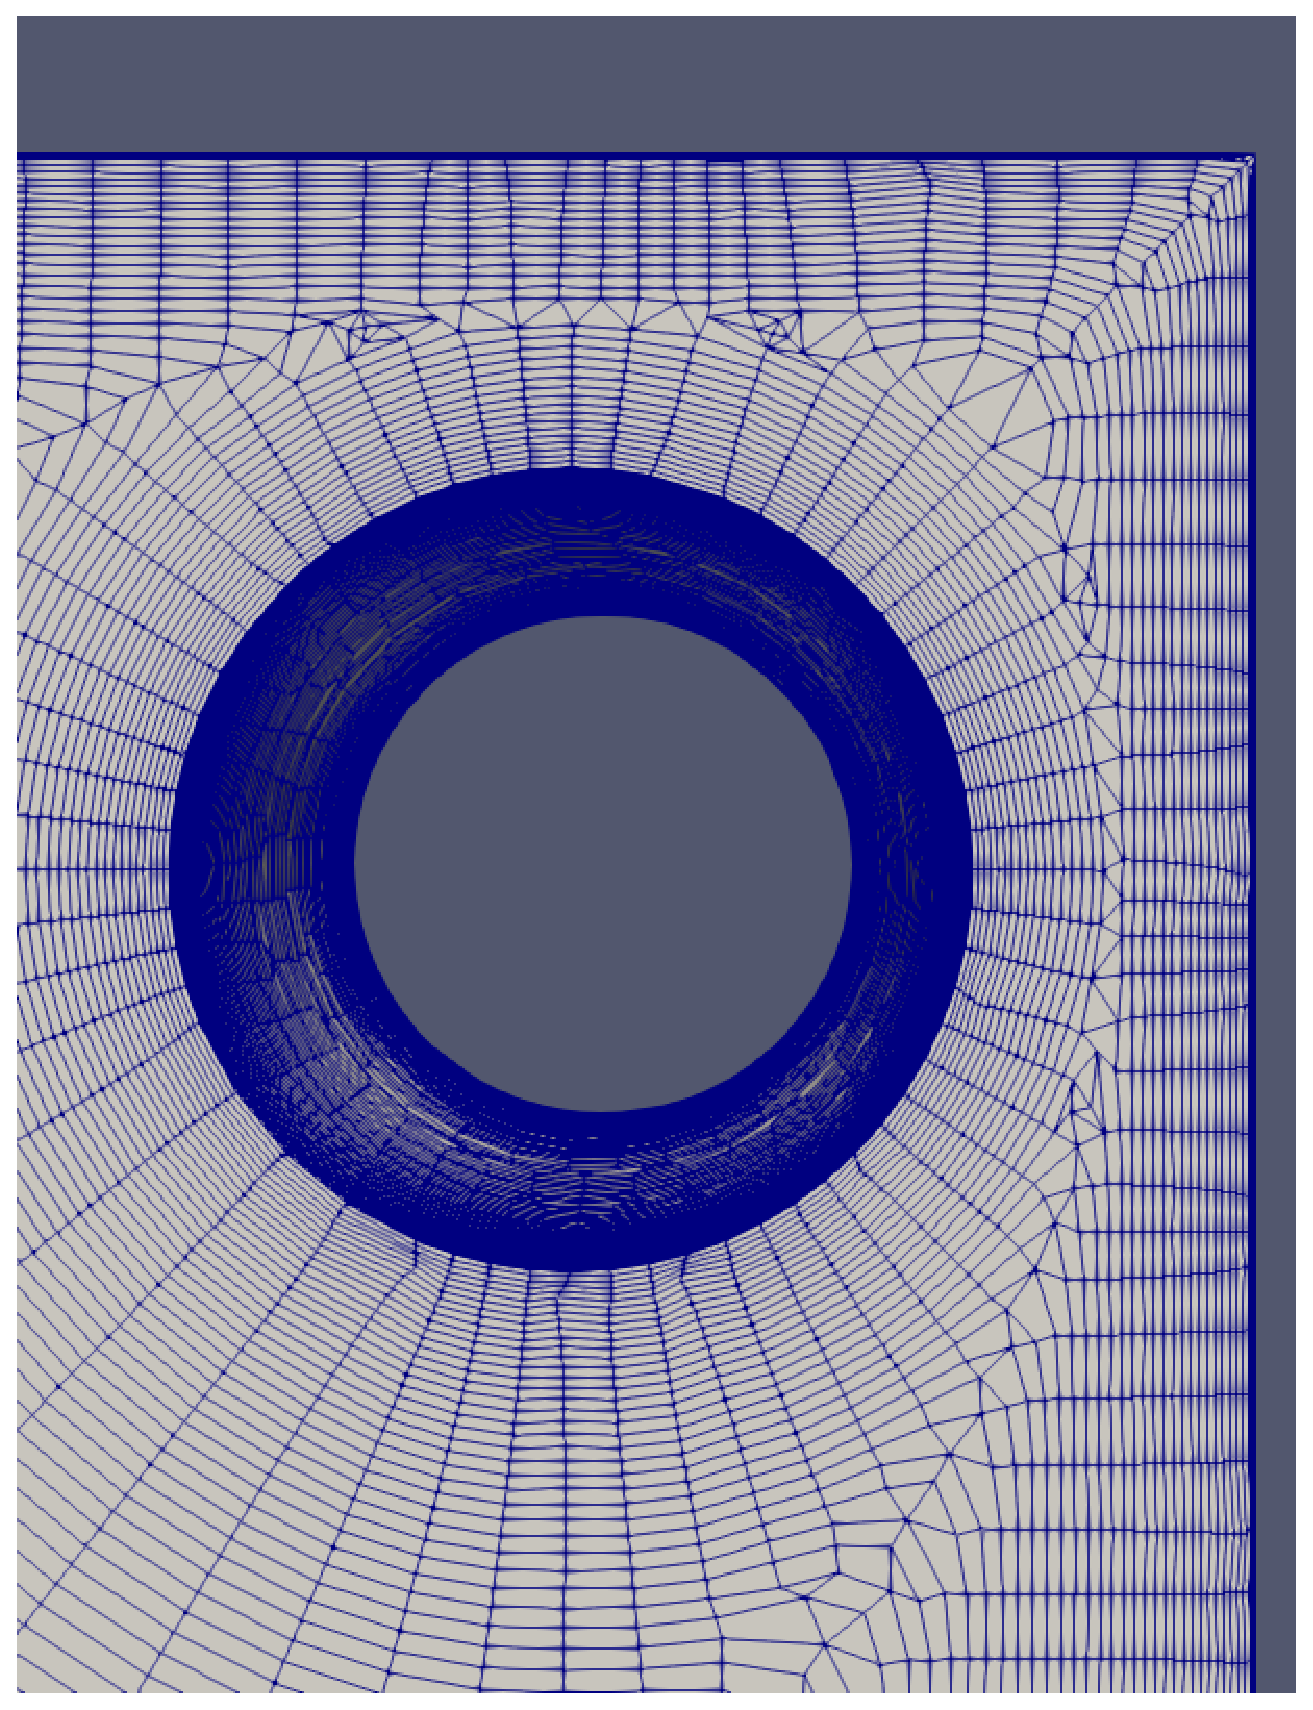
\includegraphics[width=0.9\linewidth]{img/r/joint-x0.004-g1.04-a5/bottomCloseUp.eps}
		\caption{}
		\label{closeUp2}
	\end{subfigure}
	\caption[Close up views of the meshes generated for a mechanical joint.]{Close up views of the meshes generated for a mechanical joint. (a) Close up view from the top of the mechanical joint as seen in Figure \ref{fig-joint-top}, near the region where the flat section with a cylindrical cutout meets the curved surface at the top. (b) Bottom of the part near the cylindrical cutout. Mesh layers collide at various angles in these examples. The advancing front stops marching some of its vertices using the collision handling subroutine and the algorithm continues to march the next layer on to the remaining region on the surface.}
	\label{fig-closeUp}
\end{figure}
\begin{figure}
	\centering
	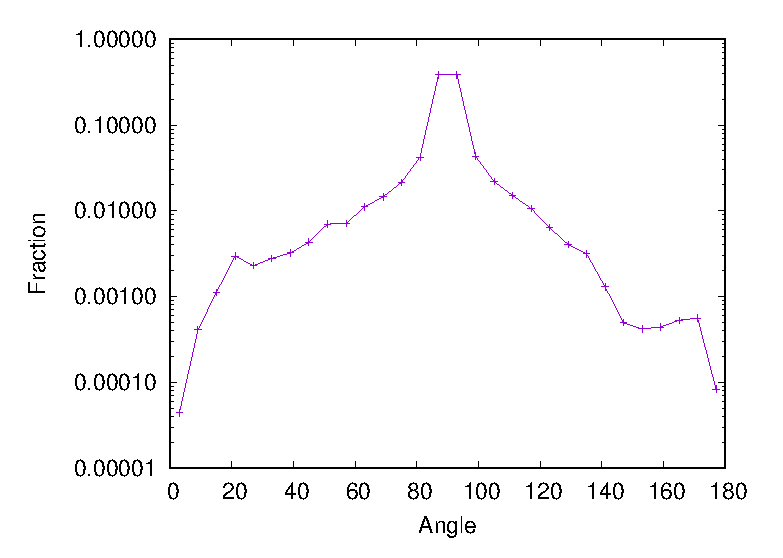
\includegraphics[width=0.5\linewidth]{img/r/joint-x0.004-g1.04-a5/jointSurfMesh.eps}
	\caption{Distribution of interior angles for the EDAMSurf mesh generated for mechanical part geometry.}
	\label{qualityJoint}
\end{figure}

We plot the distribution of interior angles of the EDAMSurf mesh produced for the mechanical part in Figure \ref{qualityJoint}. Similar to the previous test case, we have a peak near 90$^\circ$ in the plot. This is because most of the mesh elements resemble a rectangular quad. Around 0.2\% of the interior angles are less than 20$^\circ$ or greater than 160$^\circ$. This tells us that there are hardly any triangles qualify as skinny triangles in the mesh. On the other hand, 98.3\% of the interior angles are between 45$^\circ$ and 135$^\circ$. Hence, the EDAMSurf mesh contains well-shaped mesh elements.

\section{NACA0018}

In the previous two sections, we saw how EDAMSurf is capable of meshing geometries with sharp corners and diverse topology. In this section, we try to mesh a simple wing geometry. We take the NACA0018 airfoil 2D profile and extrude it in 3D. The ends of the wing are closed by a flat surface with the NACA0018 profile as its boundary curve. This gives us a three-dimensional airfoil as shown in Figure \ref{fig-naca0018}. The chord length of the airfoil is 1 and the span is 6. After generating a triangulation from the solid body using the freely available software MeshLab \cite{LocalChapterEvents:ItalChap:ItalianChapConf2008:129-136}, we import it to EDAMSurf. We mesh the geometry using our advancing layer surface mesh generation routine. The airfoil profile is segmented into four sub surfaces. Two surfaces represent the two ends of the airfoil while the other two represent the top and the bottom of the airfoil.



\begin{figure}
	\centering
	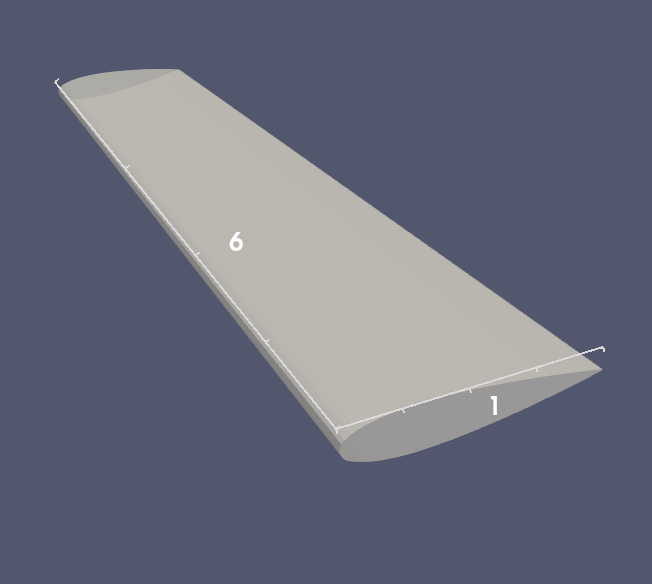
\includegraphics[width=0.6\linewidth]{img/r/naca0018.png}
	\caption{NACA0018 Airfoil profile extruded along the normal direction.}
	\label{fig-naca0018}
\end{figure}

\begin{figure}
	
	\centering
	
	\begin{subfigure}{0.4\textwidth}
		\centering
		\includegraphics[width = 0.9\linewidth, trim={0 7cm  0 7cm},clip]{img/r/naca0018-x0.007-g1.05/endCap.eps}
		\caption{}
		\label{fig-endCap-low}
	\end{subfigure}%
	\begin{subfigure}{0.4\textwidth}
		\centering
		\includegraphics[width=0.9\linewidth,trim={0 7cm  0 7cm},clip]{img/r/naca0018-x0.007-g1.1/endCap.eps}
		\caption{}
		\label{fig-endCap-high}
	\end{subfigure}
	
	\begin{subfigure}{0.4\textwidth}
		\centering
		\includegraphics[width=0.9\linewidth]{img/r/naca0018-x0.007-g1.05/oblique.eps}
		\caption{}
		\label{fig-oblique-low}
	\end{subfigure}%
	\begin{subfigure}{0.4\textwidth}
		\centering
		\includegraphics[width=0.9\linewidth]{img/r/naca0018-x0.007-g1.1/oblique.eps}
		\caption{}
		\label{fig-oblique-high}
	\end{subfigure}%
	\caption[EDAMSurf mesh for extruded NACA0018 airfoil profile.]{NACA0018 airfoil meshed with our advancing layer surface mesh algorithm. Meshes shown on the left ((a) and (c)) correspond to a growth ratio of 1.05 while ones shown on the right ((b) and (d) correspond to a growth ratio of 1.1. Anisotropic refinement of the mesh can be seen at the leading edge, trailing edge, and both end caps of the airfoil.}
	\label{fig-naca}
\end{figure}

We show two of the meshes we generate from this geometry. The first one is shown in Figure \ref{fig-endCap-low} and \ref{fig-oblique-low}. Here, we use a growth ratio of 1.05 and an initial extrusion length of 0.007. The aspect ratio value at the boundary curves ranges from 5-25. The second mesh is shown in Figure \ref{fig-endCap-high} and \ref{fig-oblique-high}. The meshes can be seen to have anisotropic refinement at the leading edge, the trailing edge and the boundary of the end caps of the airfoil. The discretization of the boundary of the airfoil is carried several layers into the surface mesh.

\begin{table}[]
	\caption{\label{table-naca} Mesh parameters for NACA0018 wing (chord length $c = 1$)}
	\centering
	\begin{tabular}{c|c|c|c|c|c}\hline
		\begin{tabular}[c]{@{}c@{}}extrusion \\ length\end{tabular} & \begin{tabular}[c]{@{}c@{}}growth \\ ratio\end{tabular} & \begin{tabular}[c]{@{}c@{}}number\\ of quads\end{tabular} & \begin{tabular}[c]{@{}c@{}}number\\ of tris \end{tabular} & \% quads & \begin{tabular}[c]{@{}c@{}}\% angles\\ between 45$^{\circ}$-135$^{\circ}$\end{tabular} \\ \hline
		0.007                                                       & 1.05                                                    & 3750                                                     & 162                                                      & 95.86 & 97.38                                                              \\
		0.007                                                       & 1.1                                                     & 2678                                                      & 198                                                       & 93.11 & 96.22               \\                                               
		\hline
	\end{tabular}
\end{table}

In the meshes generated by EDAMSurf, most of the elements are quadrilateral elements. Very few triangular elements are also present in the mesh. As discussed in Section \ref{sec-simplicial}, these triangular elements help conform to the geometry while giving more flexibility during the mesh generation process.

\begin{figure}[!hbt]
	\centering
	\begin{subfigure}{0.5\textwidth}
		\centering
		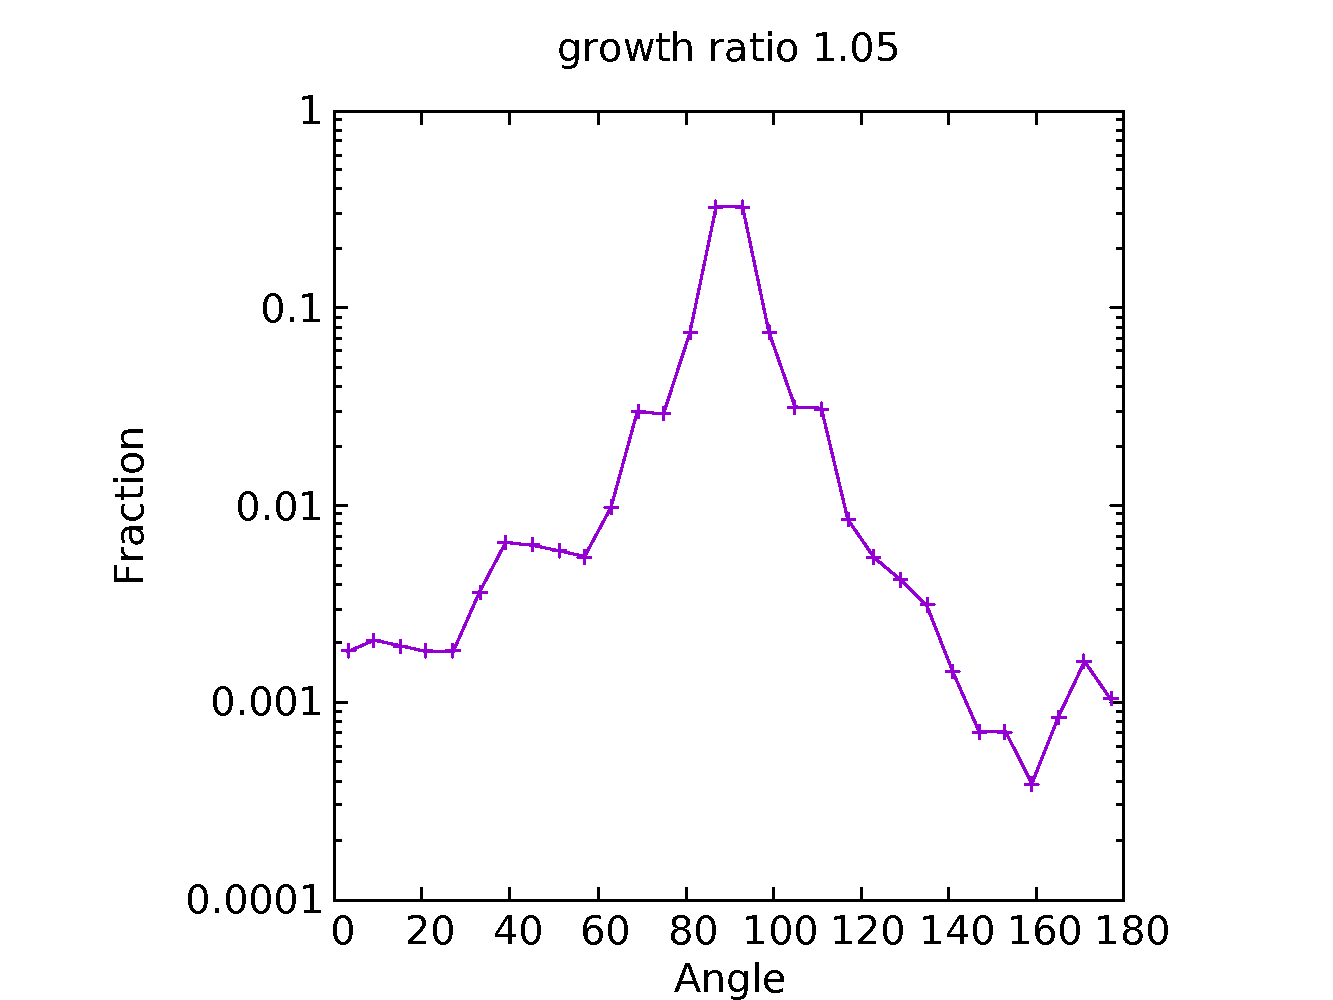
\includegraphics[width=0.9\linewidth]{img/r/naca0018-x0.007-g1.05/angleDistribution.pdf}
		\caption{}
		\label{fig-dist-low}
	\end{subfigure}%
	\begin{subfigure}{0.5\textwidth}
		\centering
		\includegraphics[width = 0.9\linewidth]{img/r/naca0018-x0.007-g1.1/angleDistribution.pdf}
		\caption{}
		\label{fig-dist-high}
	\end{subfigure}
	\caption[Interior angle distribution of EDAMSurf of NACA0018 wing geometry.]{Distribution of interior angles of the cells for the meshes generated for NACA 0018 wing. Most of the angles of the cells in the mesh are around 90$^\circ$ with a very few skinny angles.}
	\label{fig-angle-distribution}
\end{figure}

Table \ref{table-naca} shows the mesh parameters for the two cases shown in the figure. In the higher growth ratio case, 96.22\% of the angles in the mesh elements are between 45$^\circ$ and 135$^\circ$. In the mesh with the lower growth ratio, 97.38\% of the angles are in that range. In Figure \ref{fig-angle-distribution}, we plot the distribution of angles for the mesh elements in the two meshes. As can be seen from the distribution, for both the cases, most of the angles are withing a 30$^\circ$ range of 90$^\circ$. The distribution is plotted on a log scale to highlight the variation from the mean value. The distribution of angles is more spread out for the higher growth ratio case due to a higher number of triangles in that case. Only a few of the angles are close to 0$^\circ$ and 180$^\circ$. This is because of the sharp trailing edge of the geometry, which has to be dealt with using the corner collision algorithm described in Section \ref{collisionConcaveCorner}. Overall, the algorithm produces quad-dominant meshes with very few skinny cells.

This NACA0018 airfoil example shows that EDAMSurf can create stretched or anisotropic meshes for simple wing geometries. It produces a mesh consisting primarily of quadrilateral elements with a few triangular elements. Lastly, the topology of the boundary curves of the sub-surfaces is propagated several layers into the mesh.

\section{NASA Common Research Model (CRM)}

\begin{figure}[!hbt]
	\centering
	\begin{subfigure}{\textwidth}
		\centering
		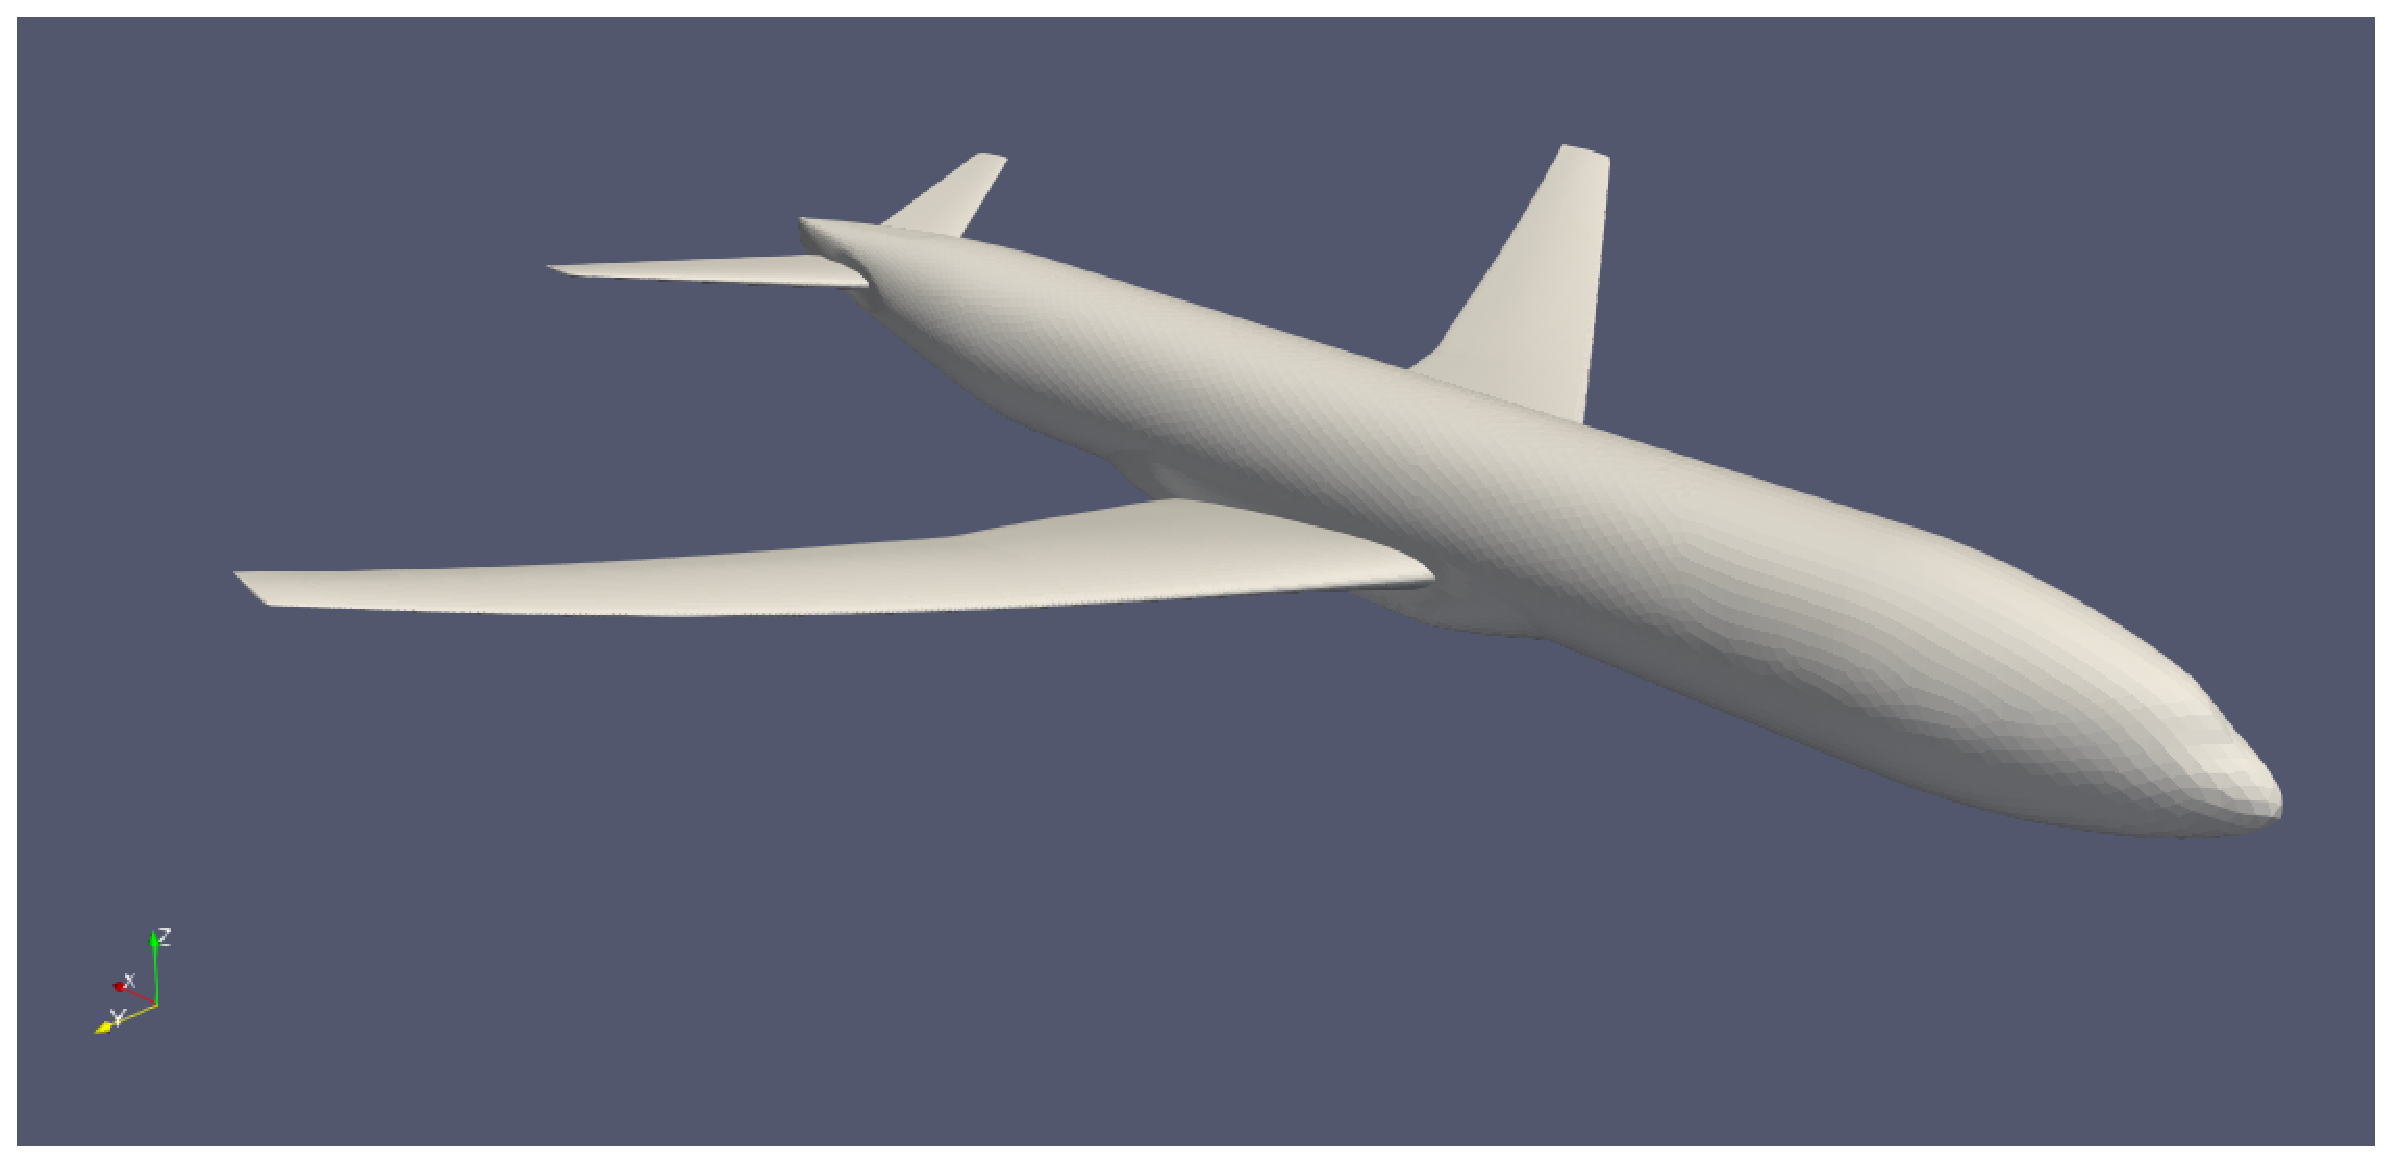
\includegraphics[trim={0 3.5cm 0 1cm},clip,width=0.88\linewidth]{img/r/dpw4/dpw4.eps}
		\caption{}
		\label{dpw4}
	\end{subfigure}
	\begin{subfigure}{0.45\textwidth}
		\centering
		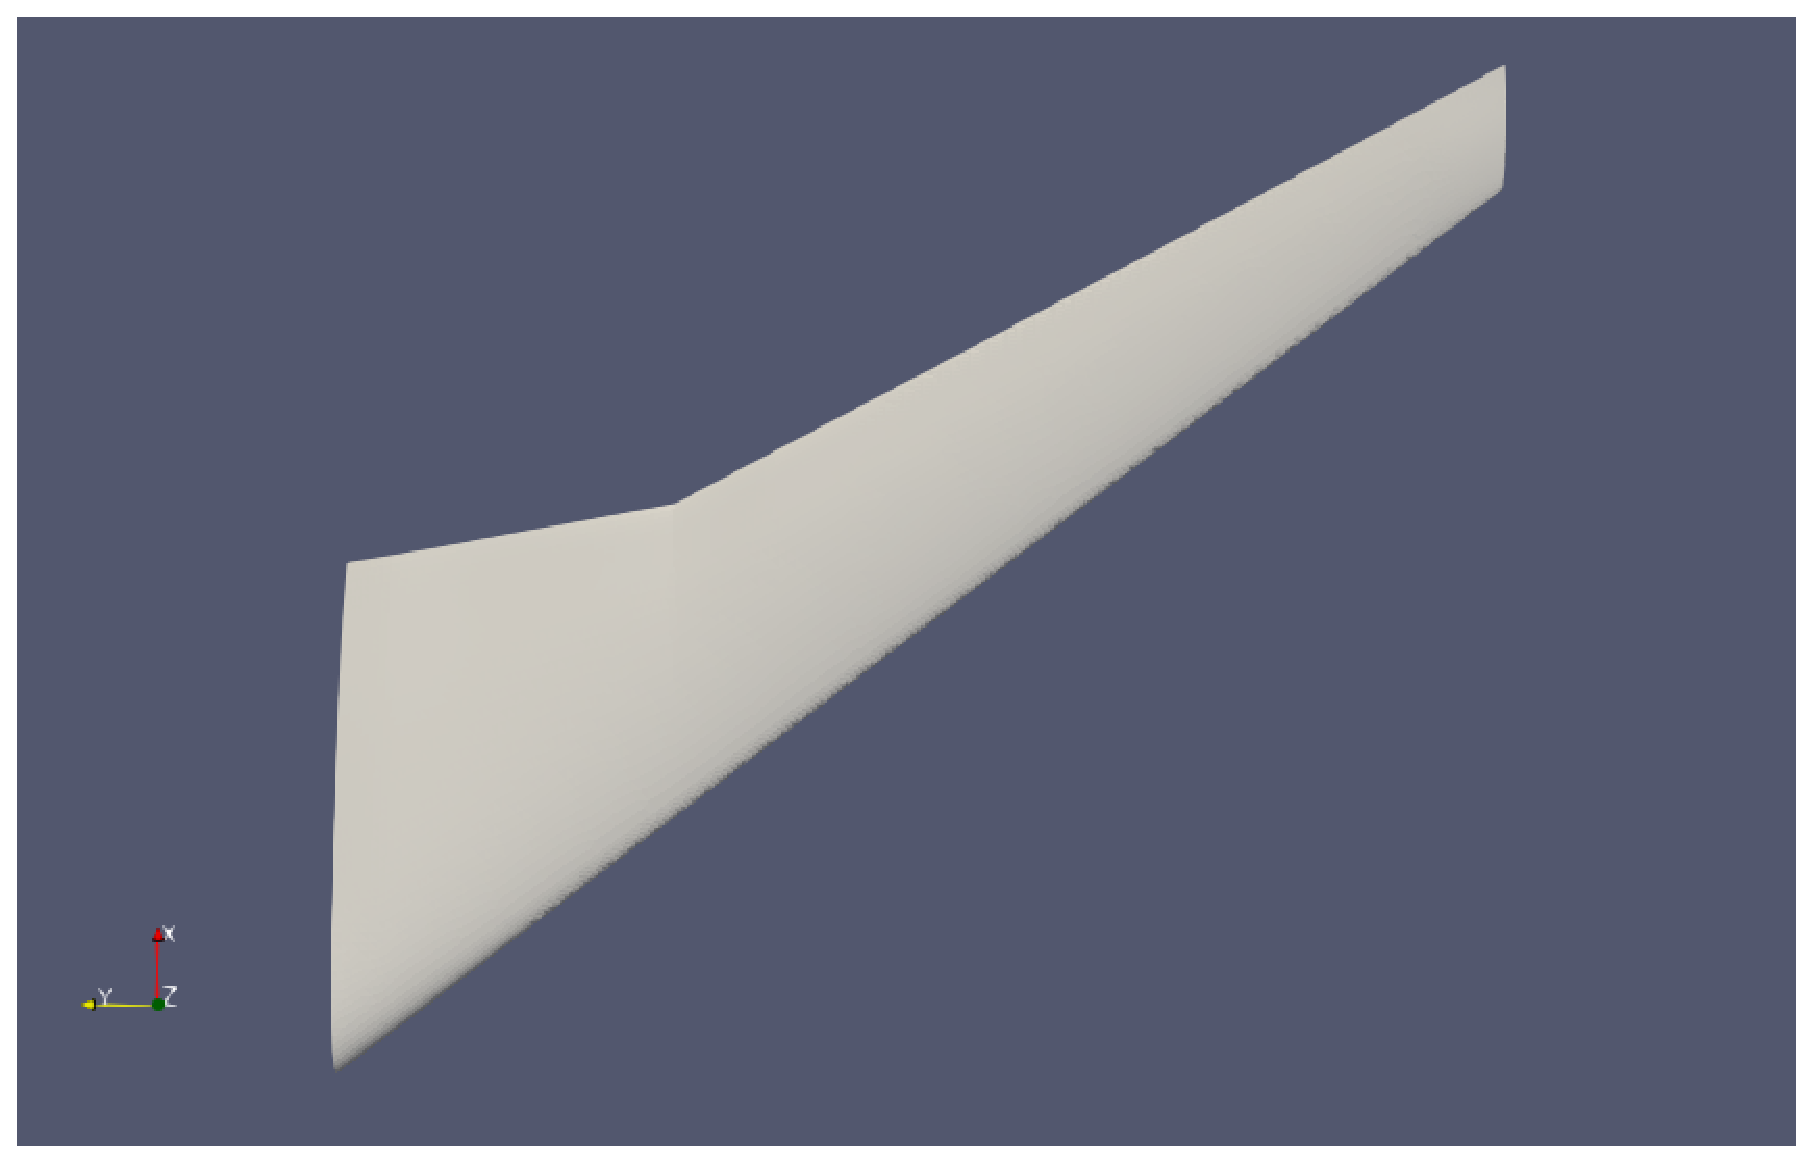
\includegraphics[width = 0.96\linewidth]{img/r/dpw4/wingTop.eps}
		\caption{}
		\label{wingTop}
	\end{subfigure}%
	\begin{subfigure}{0.45\textwidth}
		\centering
		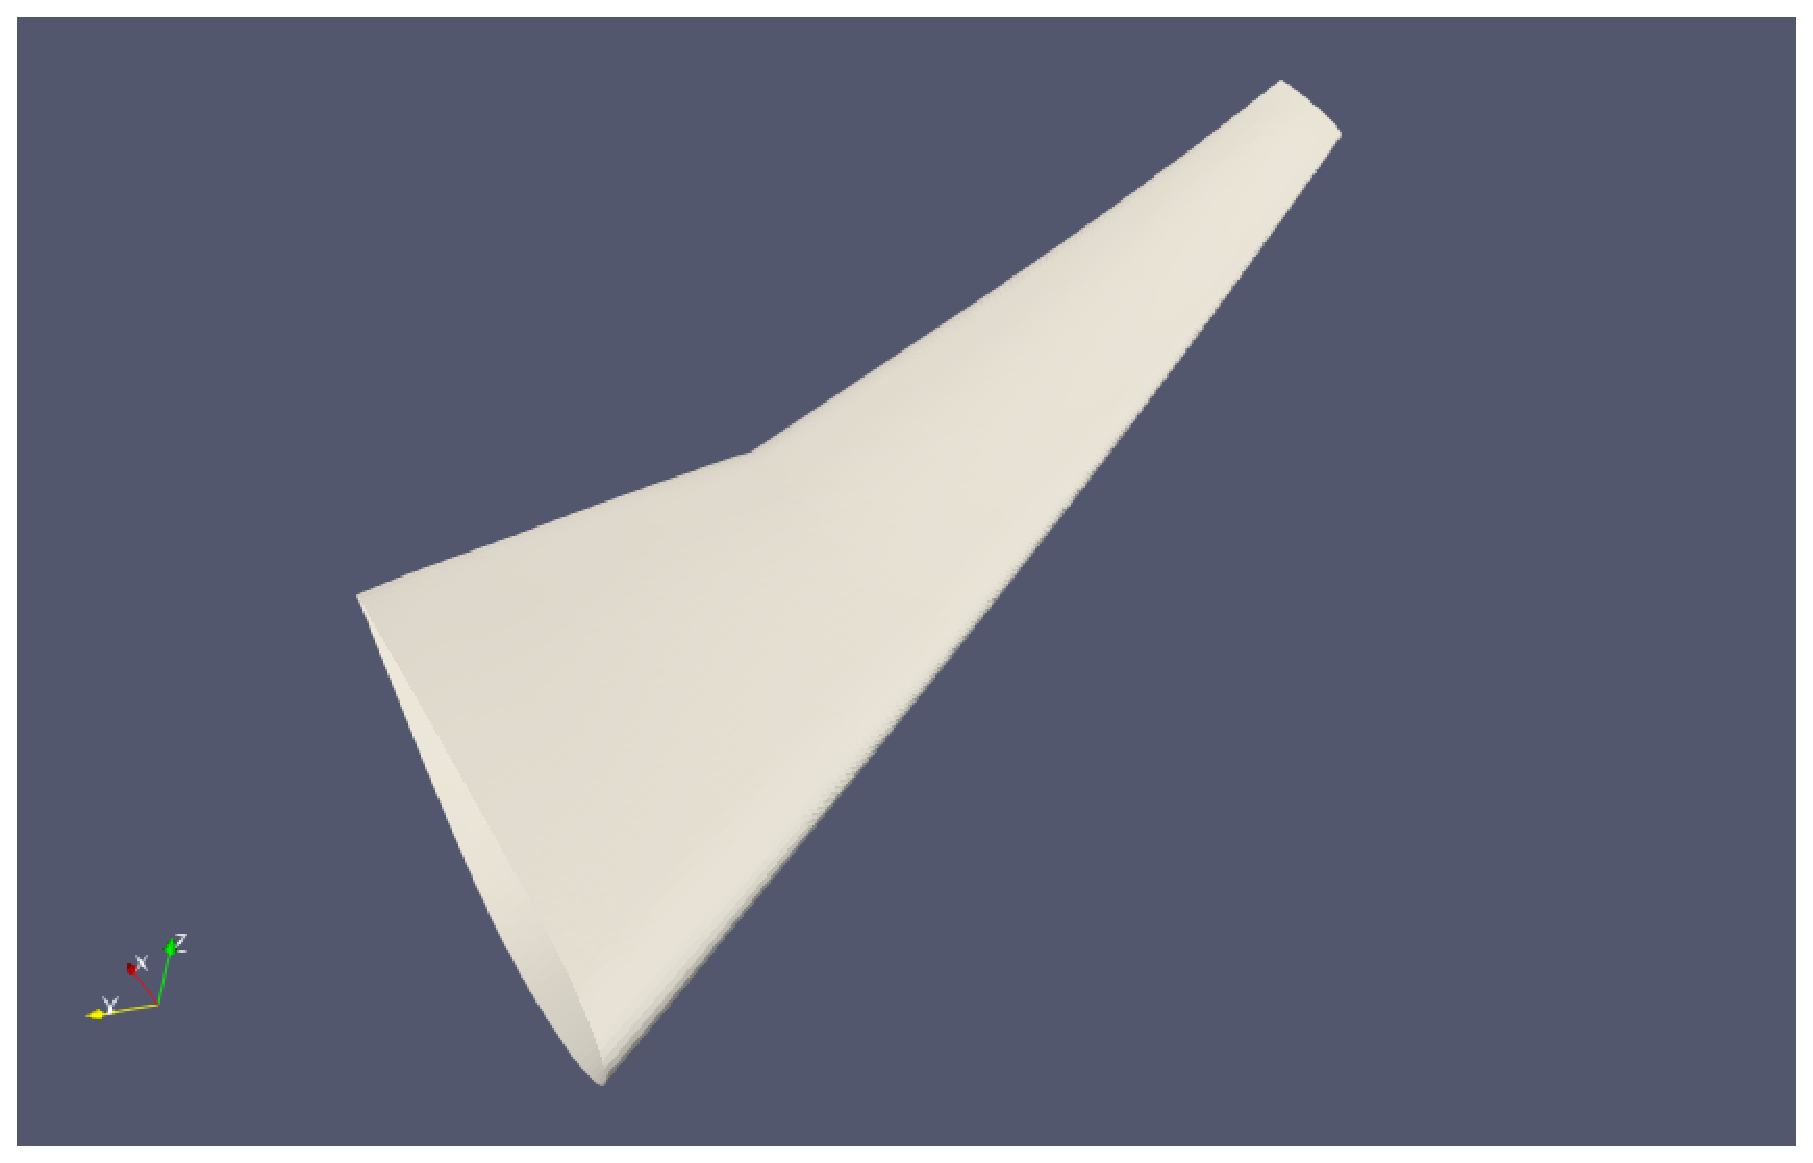
\includegraphics[width=0.96\linewidth]{img/r/dpw4/wingOblique.eps}
		\caption{}
		\label{wingOblique}
	\end{subfigure}
	\begin{subfigure}{\textwidth}
		\centering
		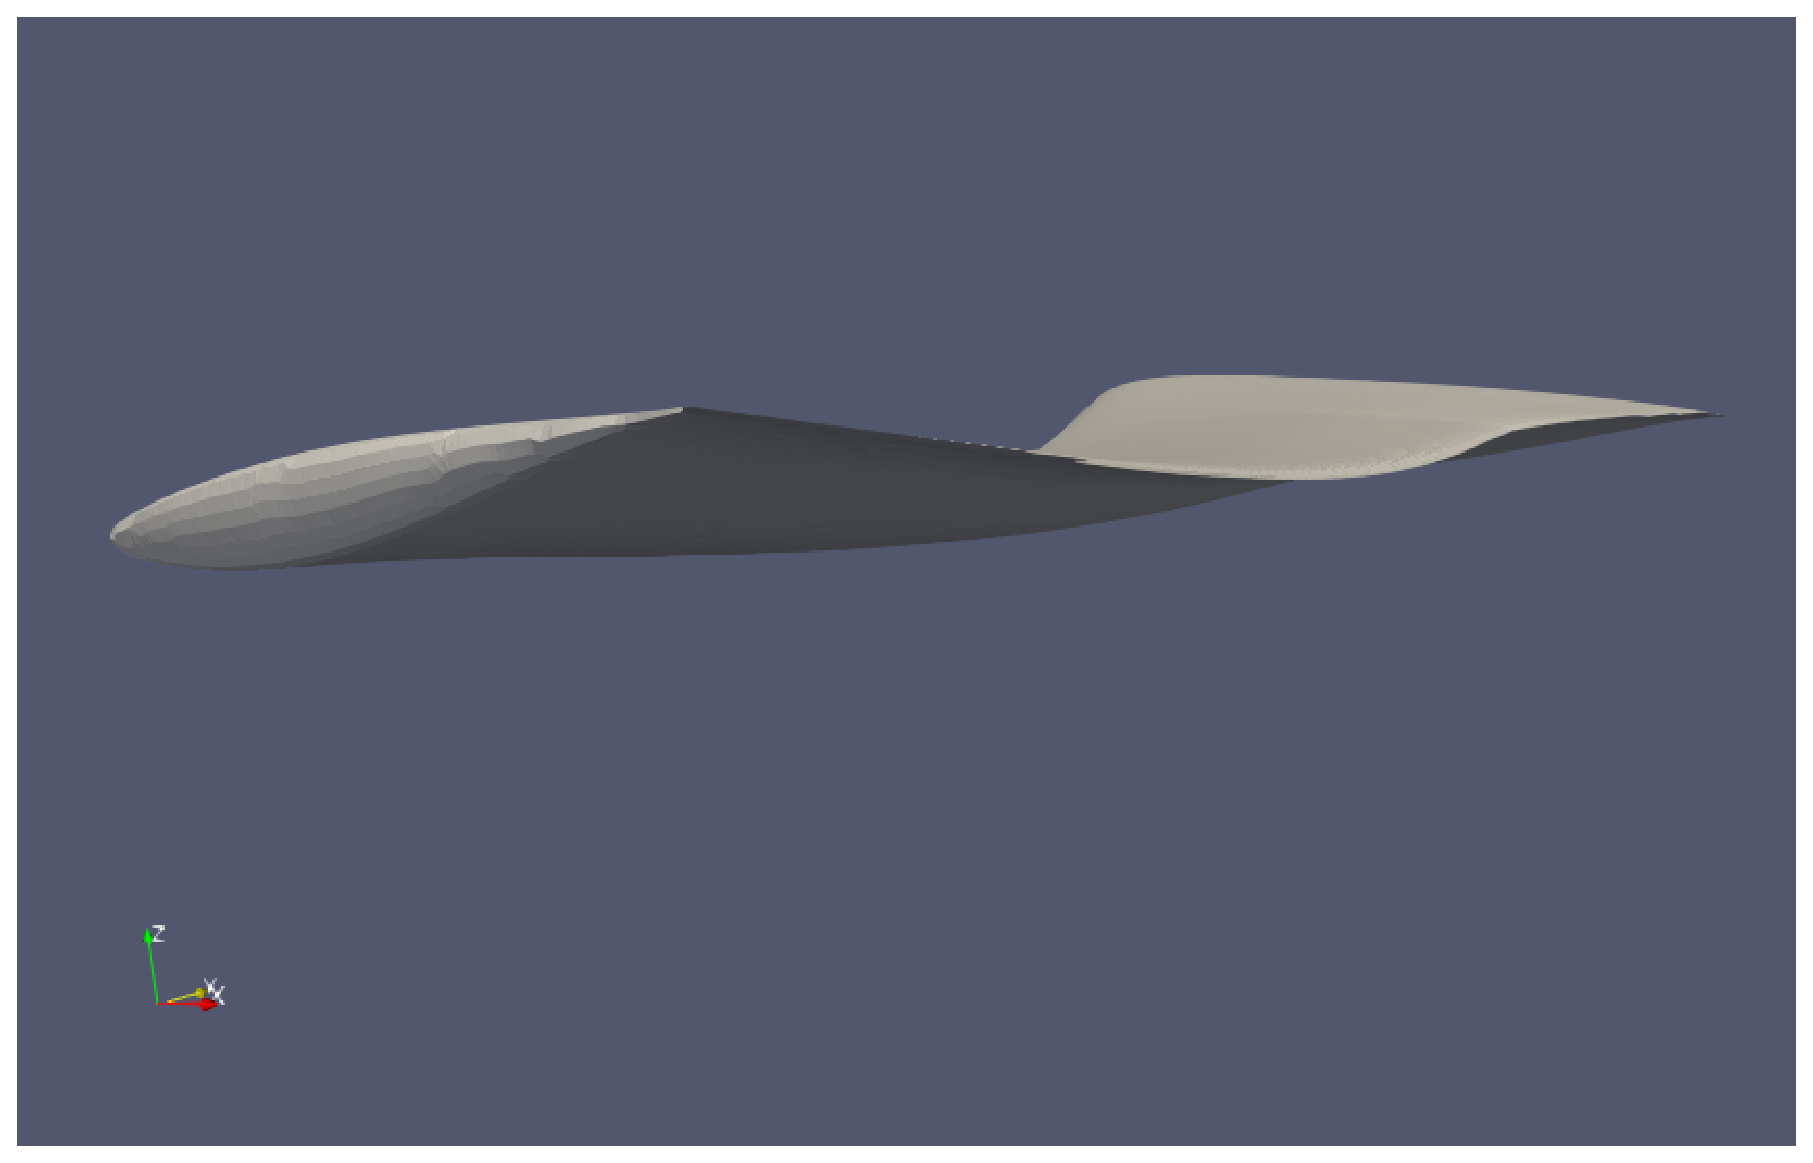
\includegraphics[width=0.88\linewidth,trim={0 8cm 0 5cm},clip]{img/r/dpw4/wingTip.eps}
		\caption{}
		\label{wingTip}
	\end{subfigure}
	\caption[Various views of NASA Common Research Model(CRM) airplane.]{(a) NASA Common Research Model, used in the 4th Design Prediction Workshop (DPW4). (b) Top view of the wing. The wing has Quarter-chord Sweep = 35$^\circ$ and a Yehudi Break at 37$\%$ of semispan. (c) Oblique view of the wing. (d) View from the side of the wing tip.}
	\label{fig-dpw4}
\end{figure}

We tested the Entire Domain Advancing Layer Surface Mesh Generation Algorithm (EDAMSurf) for robustness at the start of this chapter. Then, we showed how EDAMSurf can tackle simple wing geometries by generating a mesh for an extruded NACA 0018 airfoil profile. In this section, we pick a comparatively large, research model scaled geometry and mesh that. We pick the 4th AIAA CFD Drag Prediction Workshop's Common Research Model(CRM)\cite{vassberg2008development}. The research model was used to predict drag on it `blindly'. In other words, a priori experimental data was not given for comparison. Developed at NASA Langley Research Center, the wing of the research model was developed for well behaved aerodynamic characteristics. The aerodynamic profile of the wing offers high performance. Figure \ref{fig-dpw4} shows the research model from various views.

We segment the wing out of the Common Research Model and create the mesh on it. The wing geometry is shown in Figure \ref{wingTop}, \ref{wingOblique} and \ref{wingTip}. As the CRM wing geometry does not have sharp boundaries that could be identified by the Common Geometry Module's (CGM) facet surface import functionality, we segment the wing geometry into three sub surfaces manually before feeding them into EDAMSurf. The three sub surfaces are the upper surface of the wing, the lower surface and the end cap of the wing. 

The paper `Development of a Common Research Model for Applied CFD Validation Studies'\cite{vassberg2008development} gives detailed information regarding CRM's geometry. It also provides the Overflow isobars over the wing surface and the pressure distribution over it at the design point. The Overflow isobars can be seen in Figure \ref{fig-overflowIsobar}. The pressure distribution provided indicates that there are high pressure gradients at the leading edge and the wing tip. The gradients at the trailing edge of the wing are also reasonably high. Hence, high refinement at these regions of the wing surface is desirable in the mesh.

\begin{figure}[!hbt]
	\centering
	\begin{subfigure}{0.5\textwidth}
		\centering
		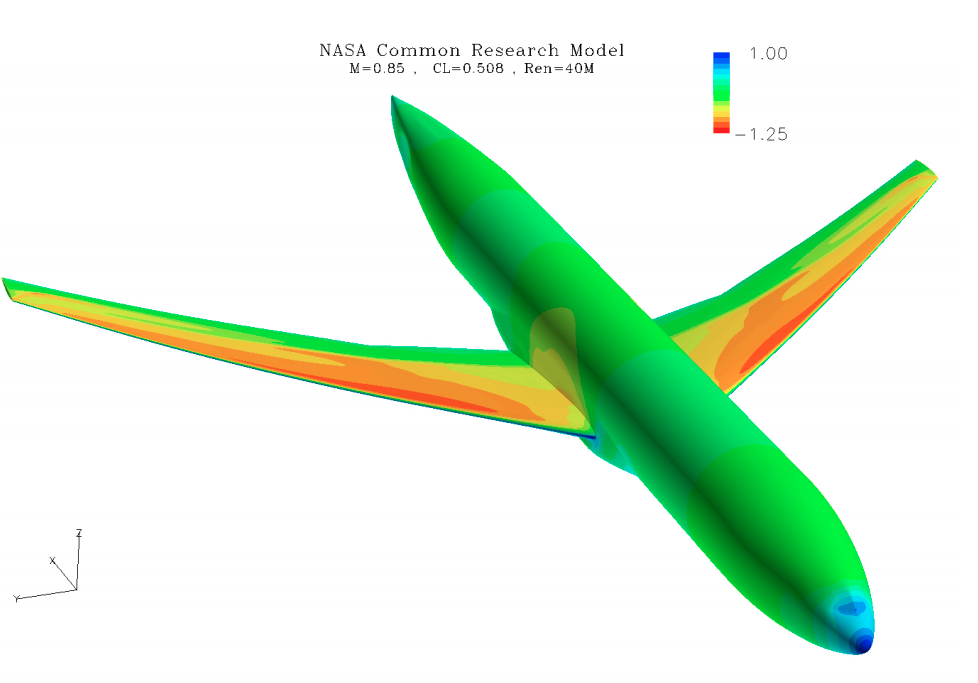
\includegraphics[width=0.9\linewidth]{img/r/dpw4/overflowIsobar.png}
		\caption{}
		\label{overflowIsobar}
	\end{subfigure}%
	\begin{subfigure}{0.5\textwidth}
		\centering
		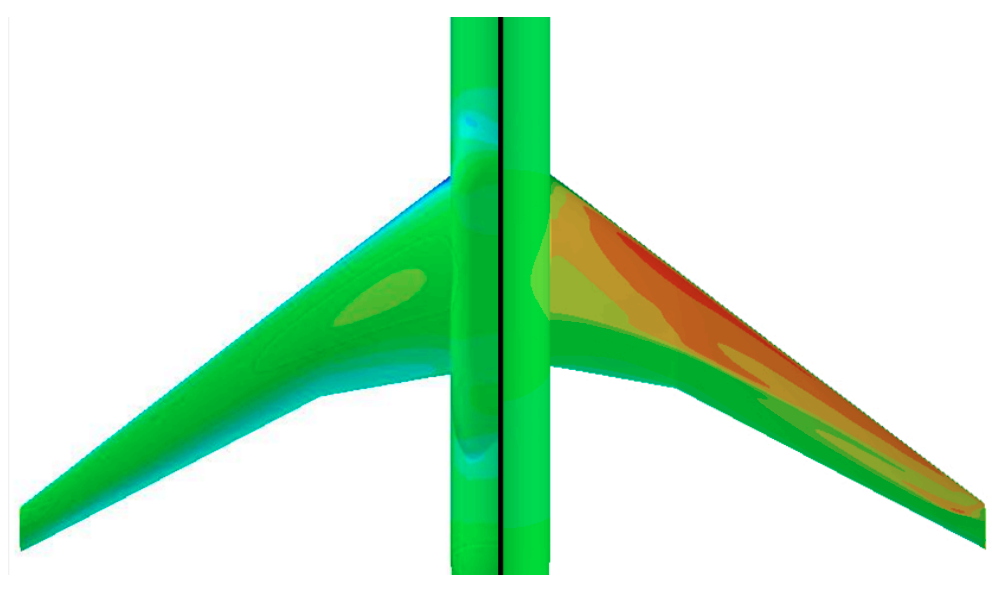
\includegraphics[width = 0.9\linewidth]{img/r/dpw4/overflowIsobar2.png}
		\caption{}
		\label{overflowIso}
	\end{subfigure}%
	\caption[Overflow Isobars of the CRM Wing/Body at the Design Point.]{Overflow Isobars of the CRM Wing/Body at the Design Point. (a) Oblique view from the top of CRM. (b) On the left, overflow isobars of the bottom surface are shown and on the right, the same is shown for the top surface. Sharp gradients can be seen near the leading edge towards the direction normal to the leading edge.}
	\label{fig-overflowIsobar}
\end{figure}


The imported triangulation contains 6464 vertices and 12441 triangles. As you can notice, the number of cells is approximately twice as much as the number of vertices. Hence, the surface mesh has high vertex connectivity. Figures \ref{fig-beforeTop} and \ref{fig-beforeTip} show the initial triangular mesh of the wing from various angles. We can notice that there is some refinement in the regions expected to have high gradients of solution variables like pressure. However, the refinement is mostly isotropic, as seen in Figure \ref{dBeforeTop}.

Figure \ref{dBeforeLeadingRoot} shows the triangulation near the leading edge of the wing at the wing root. The aspect ratio of elements near the leading edge is around 2. Hence, the anisotropy is quite low here. Figure \ref{fig-beforeTip} shows the close-up view of the triangulation near the wing tip. At the leading edge near the wing tip (Figure \ref{dBeforeLeadingTip}), we can notice higher anisotropy with an aspect ratio in the range 2-8. However, this results in skinny triangles and greater deviation from the wing surface profile.

We mesh the three sub surfaces of the CRM wing using EDAMSurf. The length of the chord at the wing root is 467.19 units. We choose an initial extrusion length of 0.4 units and a growth ratio of 1.05 to generate the mesh. This extrusion length gives us an aspect ratio value of around 10 at the boundaries of the mesh. The initial extrusion length and growth ratio are chosen to have sufficient refinement at the boundary curves of the mesh. These include the leading edge, the trailing edge, wing-body junction at the wing root, and the region near the boundary curve of the end cap of the wing.

The mesh generated by EDAMSurf for the CRM geometry can be seen in Figure \ref{fig-dpw4TopAndBottom}. Here, the top and bottom view of the mesh is shown. In other words, the mesh for the suction surface and the pressure surface of the wing is shown. It can be seen that the mesh is highly anisotropic at the boundary curves of the wing and approaches isotropy towards the interior surfaces of the wing. Highly stretched, but well-shaped quadrilateral elements are present near the boundary curves of the surface. Some triangles are also incorporated into the mesh to maintain mesh quality and tackle front collisions.

The mesh generated using EDAMSurf contains a total of 39,865 cells and 39,358 points. The number of points is approximately the same as the number of vertices. Hence, the vertex connectivity in the mesh is low. This is an advantage of a quadrilateral dominant mesh. Any vertex-based discretization would take a considerably shorter time to run on this mesh as compared to a triangular mesh with the same number of cells.

Out of the 39,865 cells, 38,738 are quadrilateral cells and the remaining 1127 are triangular cells. This means that 97.17\% of the cells in the mesh are quadrilateral.



\begin{figure}[!hbt]
	\centering
	\begin{subfigure}{\textwidth}
		\centering
		\includegraphics[trim={10cm 0 10cm 0},clip, width=0.8\linewidth]{img/r/dpw4/before/Top.eps}
		\caption{}
		\label{dBeforeTop}
	\end{subfigure}
	\begin{subfigure}{\textwidth}
		\centering
		\includegraphics[trim={0 0 0 0},clip,width = 0.8\linewidth]{img/r/dpw4/before/LeadingRoot.eps}
		\caption{}
		\label{dBeforeLeadingRoot}
	\end{subfigure}
	\caption[Input triangulation for CRM.]{Input triangulation for CRM. (a) Top view. (b) Front view at the location where leading edge meets the wing root.}
	\label{fig-beforeTop}
\end{figure}

\begin{figure}[!hbt]
	\centering
	\begin{subfigure}{\textwidth}
		\centering
		\includegraphics[trim={0 0 0 0},clip, width=0.9\linewidth]{img/r/dpw4/before/LeadingTip.eps}
		\caption{}
		\label{dBeforeLeadingTip}
	\end{subfigure}
	\begin{subfigure}{\textwidth}
		\centering
		\includegraphics[trim={0 5cm 0 10cm},clip,width = 0.9\linewidth]{img/r/dpw4/before/Tip.eps}
		\caption{}
		\label{dBeforeTip}
	\end{subfigure}
	\begin{subfigure}{\textwidth}
		\centering
		\includegraphics[trim={15cm 8cm 0 6cm},clip, width=0.9\linewidth]{img/r/dpw4/before/LeadingEdgeNearTip.eps}
		\caption{}
		\label{dBeforeLeading}
	\end{subfigure}
	\caption[Close up views of CRM's input triangulation.]{Input triangulation for CRM. (a) Oblique view of where leading edge meets the wing tip. (b) Side view showing the end cap on the wing. (c) Front view of the leading edge near the wing tip.}
	\label{fig-beforeTip}
\end{figure}

\begin{figure}[!hbt]
	\centering
	\begin{subfigure}{\textwidth}
		\centering
		\includegraphics[trim={10cm 0 10cm 0},clip, width=0.8\linewidth]{img/r/dpw4/finalMesh/Top.eps}
		\caption{}
		\label{dTop}
	\end{subfigure}
	\begin{subfigure}{\textwidth}
		\centering
		\includegraphics[trim={10cm 0 10cm 0},clip,width = 0.8\linewidth]{img/r/dpw4/finalMesh/Bottom.eps}
		\caption{}
		\label{dBottom}
	\end{subfigure}
	\caption[Top and bottom view of EDAMSurf Mesh of CRM.]{EDAMSurf Mesh of CRM. (a) Top view. (b) Bottom view.}
	\label{fig-dpw4TopAndBottom}
\end{figure}

\begin{figure}
	\centering
	\begin{subfigure}{\textwidth}
		\centering
		\includegraphics[width=\linewidth]{img/r/dpw4/finalMesh/Root.eps}
		\caption{}
		\label{dRoot}
	\end{subfigure}
	\begin{subfigure}{\textwidth}
		\centering
		\includegraphics[width=\linewidth, trim={0 5cm 0 10cm},clip]{img/r/dpw4/finalMesh/RootTip.eps}
		\caption{}
		\label{dLeadingRoot}
	\end{subfigure}    
	\begin{subfigure}{\textwidth}
		\centering
		\includegraphics[width=\linewidth]{img/r/dpw4/finalMesh/RootTrailing.eps}
		\caption{}
		\label{dRootTrailing}
	\end{subfigure}
	\caption[Close up views near wing root of EDAMSurf mesh of CRM.]{EDAMSurf Mesh for CRM showing close up views near the root of the wing. (a) Top view near the root of the wing. (b) Leading edge. (c) Trailing edge.}
	\label{fig-dpw4Root}
\end{figure}

Figure \ref{fig-dpw4Root} shows close up views of the regions of the mesh near the wing root. In Figure \ref{dLeadingRoot}, we can see the mesh at the leading edge of the airfoil near the wing root. We can see the high anisotropic refinement desired at the leading edge. The quadrilateral elements are almost rectangular everywhere. Near the region where the advancing fronts from the wing root and the leading edge collide, we can notice that the front collision algorithm is able to recover the front successfully. Figure \ref{dRootTrailing} shows the mesh near the trailing edge of the airfoil at the wing root. Here too, we can notice the highly anisotropic advancing layers at the boundary which approach isotropy far away from the boundary. Robust interior vertex removal subroutine and front recovery subroutines help in maintaining a valid advancing front after each iteration.

In Figure \ref{fig-dpw4Tip}, we show close up views at the tip of the airfoil. In Figure \ref{dLeadingTip}, we can see that the boundary curve discretization of the end cap and the top surface of the wing are the same. Anisotropy is present both in the spanwise direction of the wing as well as towards the interior surface of the end cap. This is important to capture the gradient of the solution close to the boundary curves of the surfaces. Figure \ref{dTip} shows the end cap of the airfoil. An elliptical shaped advancing front approaches towards itself and terminates at the center of the end cap. Even in such an oddly shaped surface patch, we have the majority of the elements as nearly rectangular quadrilaterals. Figure \ref{dTipRefine} shows the top view of the wing tip near the trailing edge. Here also, we can notice a high level of anisotropy at the surface boundaries. Layers growing from three different boundary curves could be seen colliding in the center of the airfoil surface. 

Lastly, we plot the interior angles of the elements in the EDAMSurf mesh of CRM. As we have seen earlier, most of the elements of the surface mesh are rectangular quad elements. Hence, the majority of the angles are around 90$^\circ$. This is seen in the angle distribution Figure \ref{fig-quality}. There is a peak near 90$^\circ$ angle. Then, we have a couple of more peaks at 45$^\circ$ and 135$^\circ$ due to the triangles present in the mesh. More than 99\% of the angles are between 45$^\circ$ and 135$^\circ$. Hence, negligible skinny angles are produced in the mesh.

\begin{figure}[!hbt]
	\centering
	\begin{subfigure}{\textwidth}
		\centering
		\includegraphics[width=\linewidth]{img/r/dpw4/finalMesh/LeadingTip.eps}
		\caption{}
		\label{dLeadingTip}
	\end{subfigure}
	\begin{subfigure}{\textwidth}
		\centering
		\includegraphics[width=\linewidth, trim={0 5cm 0 10cm},clip]{img/r/dpw4/finalMesh/Tip.eps}
		\caption{}
		\label{dTip}
	\end{subfigure}    
	\begin{subfigure}{\textwidth}
		\centering
		\includegraphics[width=\linewidth]{img/r/dpw4/finalMesh/TipRefine.eps}
		\caption{}
		\label{dTipRefine}
	\end{subfigure}
	\caption[Close up views near wing tip of EDAMSurf mesh of CRM.]{EDAMSurf Mesh for CRM showing close up views near the wing tip. (a) Wing tip near the leading edge. (b) Side view showing the mesh on the end cap of the wing. (c) Top view near the wing tip.}
	\label{fig-dpw4Tip}
\end{figure}

\begin{figure}
	\centering
	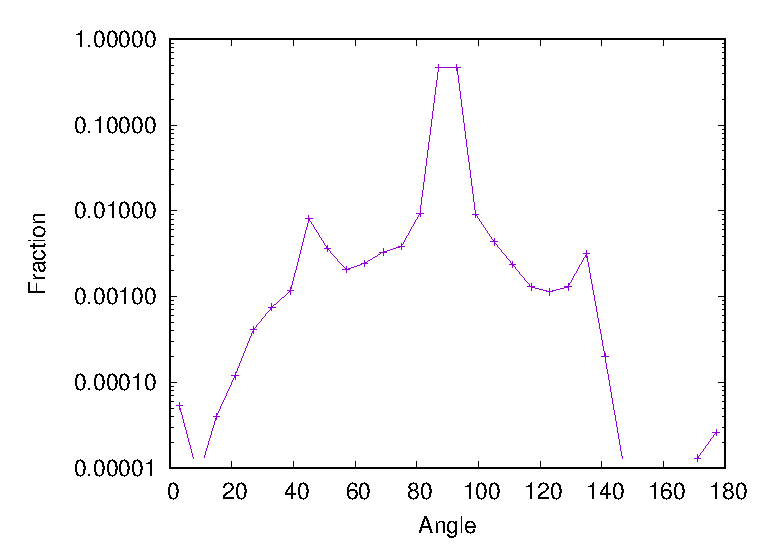
\includegraphics[width=0.8\linewidth]{img/r/dpw4/quality.eps}
	\caption[Quality of EDAMSurf mesh for CRM showing the distribution of interior angles.]{Distribution of interior angles of the elements of EDAMSurf mesh of CRM's geometry. Most of the interior angles are near the right-angled value of 90$^\circ$. Less than one percent of the angles are less than 20$^\circ$ or more than 160$^\circ$.}
	\label{fig-quality}
\end{figure}

We have seen several examples of the capabilities of EDAMSurf in this chapter. We tested the robustness of the concave angle front collision subroutine and the advancing front collision subroutine. EDAMSurf also produced desired surface meshes for geometries with diverse topologies. We also showed that EDAMSurf can handle simple airfoil geometries. We produced a mesh for NASA's Common Research Model to finish our examples. In the last chapter, we will summarize the findings of the thesis and the capabilities of EDAMSurf. We would conclude by adding some things that might be done in the future to improve the performance of EDAMSurf and to extend it in three dimensions.